\documentclass{beamer}

%% \documentclass[handout]{beamer}
%% % use this with the [handout] option to create handouts for the audience
%% \usepackage{pgfpages}
%% \pgfpagesuselayout{2 on 1}[a4paper,border shrink=5mm]

\mode<presentation>
{
  \usetheme{Diku}
% set this to your preferences:
%  \setbeamercovered{invisible}
  \setbeamercovered{transparent}
}

\usepackage{graphicx}
\usepackage{epic}

\usepackage{amsmath}
\usepackage{amssymb}
\usepackage{amsthm}

\usepackage{minibox}
\usepackage{listings}
\newcommand{\basetop}[1]{\vtop{\vskip-1ex\hbox{#1}}}
\newcommand{\source}[1]{\let\thefootnote\relax\footnotetext{\scriptsize\textcolor{kugray1}{Source: #1}}}

% for coloured code citation in text:
\usepackage{fancyvrb}

%%%%%%%%%%%%%%%%%%%%%%%%%%%%%%%%%
%%%%%    code sections   %%%%%%%%
%%%%%%%%%%%%%%%%%%%%%%%%%%%%%%%%%

% code highlighting commands in own block
\DefineVerbatimEnvironment{code}{Verbatim}{fontsize=\scriptsize}
\DefineVerbatimEnvironment{icode}{Verbatim}{fontsize=\scriptsize}

% Fancy code with color commands:
\DefineVerbatimEnvironment{colorcode}%
        {Verbatim}{fontsize=\scriptsize,commandchars=\\\{\}}

%%%%%%%%%%%%%%%%%%%%%%%%%%%%%%%%%%
%%%%%    some coloring    %%%%%%%%

\definecolor{Red}{RGB}{220,50,10}
\definecolor{Blue}{RGB}{0,51,102}
\definecolor{Yellow}{RGB}{102,51,0}
\definecolor{Orange}{RGB}{178,36,36}
\definecolor{Grey}{RGB}{180,180,180}
\definecolor{Green}{RGB}{20,120,20}
\definecolor{Purple}{RGB}{160,50,100}
\newcommand{\red}[1]{\textcolor{Red}{{#1}}}
\newcommand{\blue}[1]{\textcolor{Blue}{{#1}}}
\newcommand{\yellow}[1]{\textcolor{Yellow}{{#1}}}
\newcommand{\orange}[1]{\textcolor{Orange}{{#1}}}
\newcommand{\grey}[1]{\textcolor{Grey}{{#1}}}
\newcommand{\green}[1]{\textcolor{Green}{{#1}}}
\newcommand{\purple}[1]{\textcolor{Purple}{{#1}}}



% use "DIKU green" from our color theme for \emph
\renewcommand{\emph}[1]{\textcolor{structure}{#1}}
% use some not-too-bright red for an \emp command
\definecolor{DikuRed}{RGB}{130,50,32}
\newcommand{\emp}[1]{\textcolor{DikuRed}{ #1}}
\definecolor{CosGreen}{RGB}{10,100,70}
\newcommand{\emphh}[1]{\textcolor{CosGreen}{ #1}}
\definecolor{CosBlue}{RGB}{55,111,122}
\newcommand{\emphb}[1]{\textcolor{CosBlue}{ #1}}
\definecolor{CosRed}{RGB}{253,1,1}
\newcommand{\empr}[1]{\textcolor{CosRed}{ #1}}

\newcommand{\mymath}[1]{$ #1 $}
\newcommand{\myindx}[1]{_{#1}}
\newcommand{\myindu}[1]{^{#1}}
\newcommand{\mymathbb}[1]{\mathbb{#1}}


\newtheorem{mydef}{Definition}
\newtheorem{mytheo}{Theorem}
\newtheorem{mylemma}{Lemma}

\lstdefinelanguage{L0}
{keywords={fun,if,then,else,loop,do,map,reduce,filter,scan,redomap,mapT,reduceT,filterT,scanT,redomapT,transpose,reshape,iota,replicate,let,op,for,with},%
  sensitive=true,%
  comment=[l]{//},%
  string=[b]",%
  string=[b]'%
  basicstyle=\ttfamily\color{black},
  moredelim=**[is][\color{red}]{@}{@},
  moredelim=**[is][\color{blue}]{¤}{¤},
}

\lstset{
  language=L0
}


%%%%%%%%%%%%%%%%%%%%

%Non-Heroic AutoPar
\title[]{Scalable Conditional Induction Variables (CIV) Analysis.}

%C.~Oancea
\author[]{Cosmin E. Oancea and Lawrence Rauchwerger\\{\tt cosmin.oancea@diku.dk, rwerger@cse.tamu.edu}}

\institute{University of Copenhagen and Texas A\&M University}


\date[11/02/2015]{11th of February 2015}


\begin{document}

\titleslide


%%%%%%%%%%%%%%%%%%%%%%%%%%%%%%%%%%%%%%%%%%%%%%%%%%%%%%%%%%%%%%%%%%
%%%%%%% DOCUMENT STARTS HERE!
%%%%%%%%%%%%%%%%%%%%%%%%%%%%%%%%%%%%%%%%%%%%%%%%%%%%%%%%%%%%%%%%%%

\begin{frame}[fragile,t]
  \frametitle{Setting the Stage}

Low-level analysis of array subscripts typically assumes\\
subscripts to be affine expressions of loop indices.
\medskip

%\begin{block}{Approach Centered on Extracting Arbitrarily Shaped Predicates:} 
\begin{columns}
\column{0.33\textwidth}
\begin{colorcode}[fontsize=\small]
k = 0
DO i = 1, N
  \emp{k} = \emp{k} + 2
  \purple{A(k)} = ...
ENDDO
\end{colorcode}

\begin{itemize}
    \item \emp{Loop-carried dependences on {\tt k}},
    \item \purple{Any Dependences on {\tt A}?}
\end{itemize}

\column{0.1\textwidth}\pause
Ind\\
Var\\
$\Longrightarrow$\\
Subst
\column{0.52\textwidth}\pause
\begin{colorcode}[fontsize=\small]
k = 0
DO i = 1, N
  \emphh{A(2*i)} = ...
ENDDO
k = MAX(0,2*N)
\end{colorcode}

\begin{itemize}
    \item substituting {\tt k}$\rightarrow${\tt 2*i}:
    \item[1] eliminates \emp{dependences on {\tt k}}
    \item[2] allows easy reasoning for {\tt A}: 
                \emphh{$i_1 \neq i_2 \ \Rightarrow \ 2*i_1 \neq 2*i_2$}
\end{itemize}
\end{columns}

\end{frame}



\begin{frame}[fragile,t]
  \frametitle{Problem Statement \& Related Work}

Challenging case of subscripts using
            \emp{``conditional induction variables''} {\sc civ}: 
            monotonic, but conditionally incremented 
            (NO closed-form sol).
%    \item also effectively supported in practice.
\medskip

Filter, scan, push vector abstractions create {\sc civ} patterns.\\\smallskip
Five out of thirty ($\sim17\%$) benchmarks require {\sc civ} analysis.

\begin{columns}
\column{0.38\textwidth}
\begin{colorcode}[fontsize=\small]
civ = 0
DO i = 1, N
  \emp{IF ( B(i).GT.0 ) THEN}
    \emp{civ = civ + 1}
    A(civ) = ...
  \emp{ENDIF} 
ENDDO
\end{colorcode}
\column{0.59\textwidth}\pause
\medskip

\emphh{\em Related work:} specialized dependency test (at pair-of-accesses level)\smallskip
\begin{itemize}
    \item consecutively-written, single-index access pattern [Lin,Padua]\smallskip
    \item accesses of shape {\tt \{X(civ), X(civ+K)\}} [Wu,Cohen,Padua]\smallskip
    \item assume that {\sc civ} used only to index $\Rightarrow$
            {\sc civ} computed at the end of loop.
% pair of accesses of (above) shape are disambiguated by 
% reasoning in terms of the (range of the) cross-iteration 
% evolution of the corresponding CIV
\end{itemize}
\end{columns}

\end{frame}


\begin{frame}[fragile,t]
  \frametitle{Problem Statement \& Our Approach}

Challenging case of subscripts using
            ``\emp{conditional} induction variables'', i.e., 
            monotonic, but conditionally incremented 
            (NO closed-form sol).
%    \item also effectively supported in practice.
\bigskip

\begin{columns}
\column{0.33\textwidth}
\begin{colorcode}[fontsize=\small]
civ = 0
DO i = 1, N
  \emp{IF ( B(i).GT.0 )} 
  THEN
    \emp{civ = civ + 1}
    A(civ) = ...
  \emp{ENDIF}
ENDDO
\end{colorcode}
\column{0.69\textwidth}
\medskip

\emphh{Key difference:} 
        see it as a summarization of array references problem
\begin{itemize}

    \item {\sc civ} monotonicity $\Rightarrow$ summary monotonicity (?)
%    \item enabled by a flexible notion of monotonicity
%            of the summary,

    \item constructive rather than existential proof,

    \item common representation for affine and {\sc civ}-based summary,

    \item dependency test is modeled as an equation on 
            summaries \& requires no modification,

   \item summary-based techniques better suited for larger loops.
\end{itemize}
\end{columns}

\end{frame}


\begin{frame}[fragile,t]
  \frametitle{Problem Statement: CIV computation}

\begin{itemize}
    \item[\emp{1}] \emp{How to compute {\sc civ}s in parallel?}
%    \item[2] (How to summarize {\sc civ}-based subscripts? -- next!)
%    \item[3] (How to disambiguate {\sc civ}-based subscripts? -- next!)
\end{itemize}
\bigskip\pause

\begin{columns}
\column{0.37\textwidth}
\begin{colorcode}[fontsize=\small]
civ = civ0;
DO i = 1, N
  \emp{IF ( B(i).GT.0 ) THEN}
    \emp{civ = civ \mymath{\oplus} 1}
    A(civ) = ...
  \emp{ENDIF} 
ENDDO
\end{colorcode}
\column{0.61\textwidth}%\pause
Conceptually, parallel {\sc civ} computation is:\\
\begin{colorcode}[fontsize=\small]
X \mymath{\leftarrow} \emphh{map}(\mymath{\backslash}b\mymath{\rightarrow}\emp{if b > 0 then 1 else 0}, B)
y \mymath{\leftarrow} \emphh{scan}\mymath{\myindu{exc}}(\mymath{\oplus}, n\mymath{\myindx{el}}, X)
in \emphh{map}((\mymath{\oplus} civ0), Y)
\end{colorcode}
$\oplus$: any associative operator,\\
$n_{el}$ its neutral element.\\
\medskip
\emphh{Also solves the cases when {\tt civ} is {\bf not} used for indexing!}
\end{columns}
\bigskip
\bigskip
%\pause

\emphh{map}(f, \{$a_1$, $a_2$, $\ldots$, $a_n$\}) $\equiv$ \emph{\{f($a_1$), f($a_2$), $\ldots$, f($a_n$)\}}
\medskip

\emphh{scan$^{exc}$}($\odot$, $e$, \{$a_1$, $a_2$, $\ldots$, $a_n$\}) $\equiv$ \emph{\{$e$, $e \odot a_1$, $\ldots$, $e \odot a_1 \ldots \odot a_{n-1}$\}}

\end{frame}



\begin{frame}[fragile,t]
  \frametitle{Problem Statement: Summary Computation}

\begin{itemize}
%    \item[1] (How to compute {\sc civ}s in parallel? -- done!)
    \item[\emp{2}] \emp{How to summarize {\sc civ}-based subscripts?}
%    \item[3] (How to disambiguate {\sc civ}-based subscripts? -- next!)
\end{itemize}

%  \emphh{\mymath{\leftarrow}civ\mymath{\myindx{\mu}\myindu{i}} = }             
%  \emphh{\mymath{\leftarrow}civ\mymath{\myindx{b}\myindu{i}}}
%  {\tt civ@2 = civ@3 = civ@4}, hence 

\begin{columns}
\column{0.35\textwidth}
\begin{colorcode}[fontsize=\small]
\emp{civ@1 = civ0}
DO i = 1, N
  \emp{civ@2=\mymath{\gamma}(civ@1,civ@4)}
  IF ( B(i).GT.0 ) THEN
    \emp{civ@3 = civ@2 + 1}
    A(\emphh{civ@3}) = ...
  ELSE

  ENDIF
  \emp{civ@4=\mymath{\gamma}(civ@1,civ@4)}
ENDDO
\emp{civ@5 = \mymath{\gamma}(civ@4,civ@1)}
\end{colorcode}
\column{0.61\textwidth}%\pause
\begin{itemize}
    \item[1] gated SSA representation\pause
    \item {\sc civ} evolution on each path known $\Rightarrow$
    \item[2] express each path summary in terms of {\tt civ@2} and {\tt civ@4}
    \begin{itemize}
        \item[a] {\tt then}: {\tt \{civ$_3$\}$\equiv$\emphh{[civ@2+1,civ@4]}}\pause
        \item[b] {\tt else}: {\tt $\emptyset$ $\equiv$ \emphh{[civ@2+1,civ@4]}},
                    because {\tt civ@2+1 > civ@4}.
    \end{itemize}\pause
    \item[3] Iteration: $W_i = $\emphh{\tt{}[civ@2+1,civ@4]}\\
            (all paths identical formula).
    \item[4] Loop: $\cup_{i=1}^{N} W_i = $ \emphh{\tt{}[civ@1+1,civ@5]}\pause
    \item[5] $\cup_{k=1}^{i-1} W_k = $ \emphh{\tt{}[civ@1+1,civ@4$^{i-1}$]}\\
             $\mbox{~~~~~~~~~~~}=$ \emphh{\tt{}[civ@1+1,civ@2$^{i}$]}
\end{itemize}
\end{columns}
\bigskip
\bigskip
%\pause

\end{frame}

\begin{frame}[fragile,t]
  \frametitle{Problem Statement: Independence Equations}

\begin{itemize}
%    \item[1] (How to compute {\sc civ}s in parallel? -- done!)
%    \item[2] (How to summarize {\sc civ}-based subscripts? -- done!)
    \item[\emp{3}] \emp{How to disambiguate {\sc civ}-based subscripts?}
\end{itemize}

%  \emphh{\mymath{\leftarrow}civ\mymath{\myindx{\mu}\myindu{i}} = }             
%  \emphh{\mymath{\leftarrow}civ\mymath{\myindx{b}\myindu{i}}}
%  {\tt civ@2 = civ@3 = civ@4}, hence 

\begin{columns}
\column{0.35\textwidth}
\begin{colorcode}[fontsize=\small]
\emp{civ@1 = civ0}
DO i = 1, N
  \emp{civ@2=\mymath{\gamma}(civ@1,civ@4)}
  IF ( B(i).GT.0 ) THEN
    \emp{civ@3 = civ@2 + 1}
    A(\emphh{civ@3}) = ...
  ELSE

  ENDIF
  \emp{civ@4=\mymath{\gamma}(civ@1,civ@4)}
ENDDO
\emp{civ@5 = \mymath{\gamma}(civ@4,civ@1)}
\end{colorcode}
\column{0.61\textwidth}%\pause
\begin{itemize}
    \item[1] Loop independence by set equations:\smallskip
    \item Output independence: $\cup_{i=1}^{n}(\ \cup_{k=1}^{i-1}W_k \ \cap \ W_i ) \ = \emptyset$\smallskip\pause
    \item $\cup_{i=1}^{n}($ {\tt[civ@1+1,civ@2$^{i}$] $\cap$}\\
          $\mbox{~~~~~~~~}${\tt[civ@2$^{i}$+1,civ@4$^{i}$]$~~) = \emptyset$}\bigskip
    \item[2] Other uses: per-iteration copy-in/out
\end{itemize}
\end{columns}
\bigskip
\bigskip
%\pause

\end{frame}

\begin{frame}[fragile,t]
\frametitle{A Nontrivial Loop: {\tt CORREC\_do401} {\scriptsize(BDNA,PERFECT-CLUB)}}

\begin{columns}
\column{0.44\textwidth}
\begin{colorcode}[fontsize=\small]
civ@1 = Q
DO i = M, N, 1
 civ@2=\mymath{\gamma}(civ@1,civ@4)
 .. = {\bf X}(\emp{i}) ..
 IF C(i) .GT. 0 THEN
  DO j = 1, C(i), 1
   \purple{IF(..)}{\bf{}X}(\emp{j+civ@2       })=..
   \purple{IF(..)}{\bf{}X}(\emp{j+civ@2+  C(i)})=..
   \purple{IF(..)}{\bf{}X}(\emp{j+civ@2+2*C(i)})=..
  ENDDO
  \blue{civ@3 = 3*C(i) + civ@2}
 ENDIF
 civ@4=\mymath{\gamma}(civ@3,civ@2)
ENDDO
civ@5=\mymath{\gamma}(civ@4,civ@1)
\end{colorcode}
\column{0.54\textwidth}%\pause
\begin{itemize}
    \item \blue{{\sc civ} may have non-constant evolution through loop}\pause\medskip
    \item \emp{{\sc civ} subscripts:} 
        \begin{itemize}
            \item neither single indexed 
            \item nor consecutively written, 
            \item nor of shape:\\ 
                    {\tt \{X(civ), X(civ+K)\}}
        \end{itemize}\pause\medskip
    \item \purple{summary may contain holes $\Rightarrow$ over/underestimate approx.}
\end{itemize}
\end{columns}
\end{frame}

\begin{frame}[fragile,t]
\frametitle{Preliminaries: Exact USR Summarization (1)}

Summaries ({\sc ro}, {\sc rw}, {\sc wf}) are
\begin{itemize}
    \item constructed via a bottom-up parse of the \textsc{AbSyn},
    \item structural data-flow equations dictate how to compose consecutive regions,
            aggregate/translate across loops/callsites, ...
\end{itemize}
\bigskip

\begin{columns}
\column{0.44\textwidth}
\begin{colorcode}[fontsize=\small]
   \purple{IF(..)}{\bf{}X}(j+civ@2       )=..
   \purple{IF(..)}{\bf{}X}(j+civ@2+  C(i))=..
   \purple{IF(..)}{\bf{}X}(j+civ@2+2*C(i))=..
\end{colorcode}
\column{0.54\textwidth}%\pause
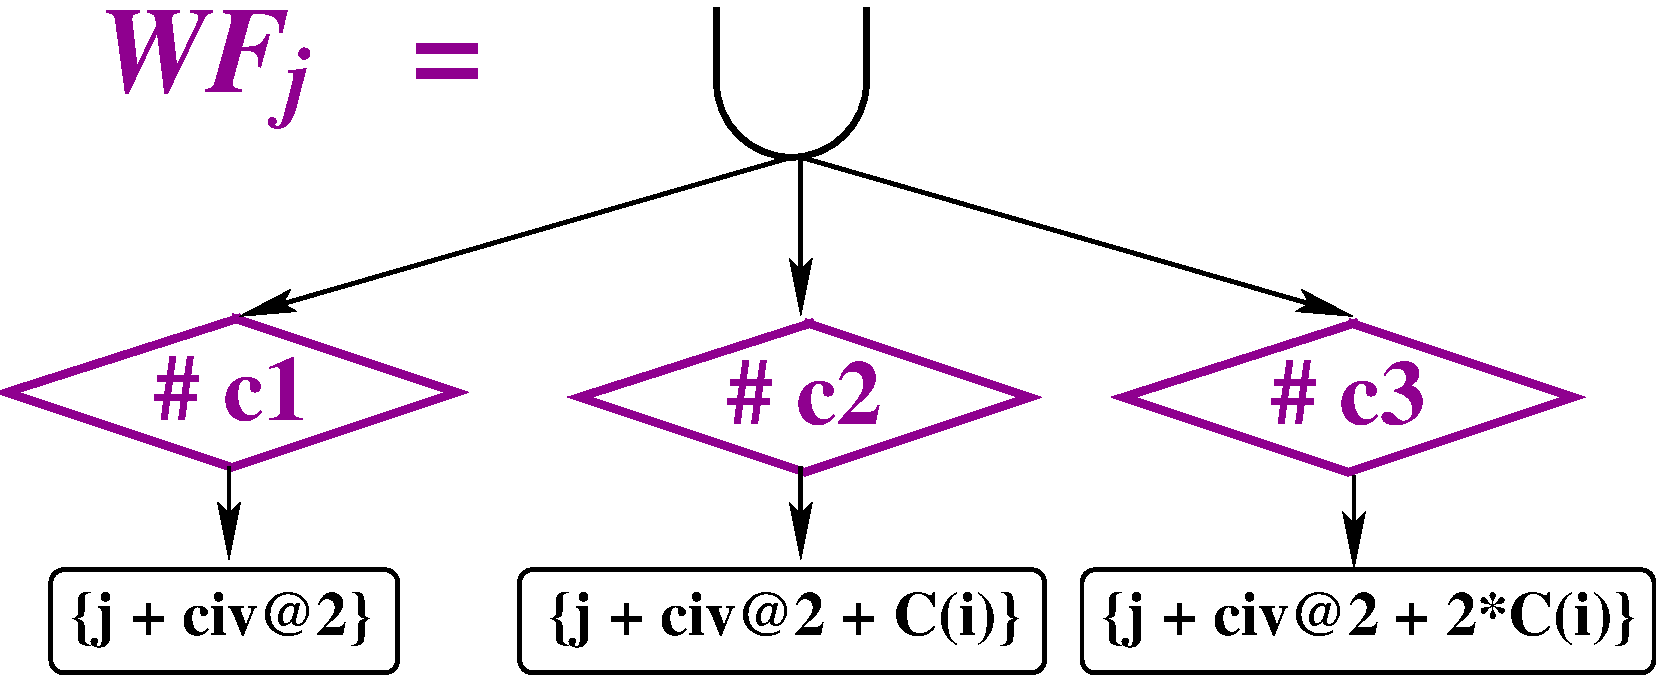
\includegraphics[height=15ex]{Figures/WFj_USR}
\end{columns}

\end{frame}

\begin{frame}[fragile,t]
\frametitle{Preliminaries: Exact USR Summarization (2)}

\bigskip

\begin{columns}
\column{0.38\textwidth}
\begin{colorcode}[fontsize=\small]
  \blue{DO j = 1, C(i), 1}
   \purple{IF(..)}{\bf{}X}(j+civ@2       )=..
   \purple{IF(..)}{\bf{}X}(j+civ@2+  C(i))=..
   \purple{IF(..)}{\bf{}X}(j+civ@2+2*C(i))=..
  \blue{ENDDO}
\end{colorcode}
\column{0.59\textwidth}%\pause
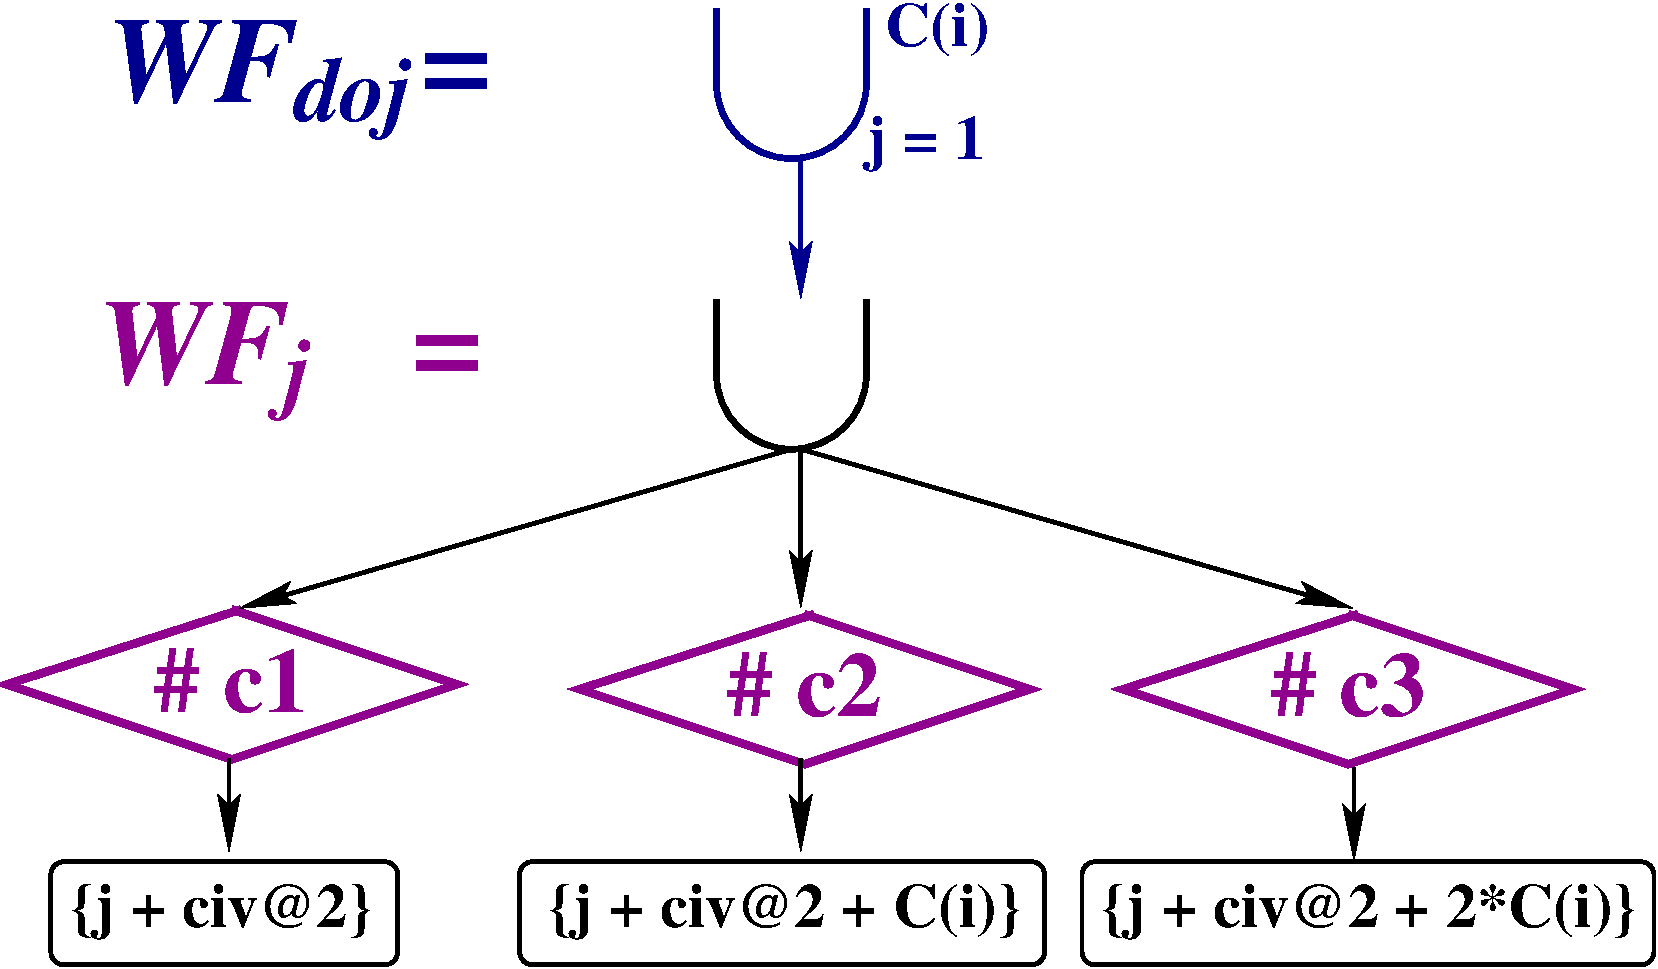
\includegraphics[height=25ex]{Figures/WFdoj_USR}
\end{columns}

\end{frame}


\begin{frame}[fragile,t]
\frametitle{Preliminaries: Exact (USR) Summarization (3)}

\begin{columns}
\column{0.34\textwidth}
\begin{colorcode}[fontsize=\small]
 \emp{IF C(i) .GT. 0 THEN}
  \blue{DO j = 1, C(i), 1}
   \purple{IF(..)}{\bf{}X}(j+civ@2       )=..
   \purple{IF(..)}{\bf{}X}(j+civ@2+  C(i))=..
   \purple{IF(..)}{\bf{}X}(j+civ@2+2*C(i))=..
  \blue{ENDDO}
  civ@3 = 3*C(i) + civ@2
 \emp{ENDIF}
\end{colorcode}
\column{0.64\textwidth}%\pause
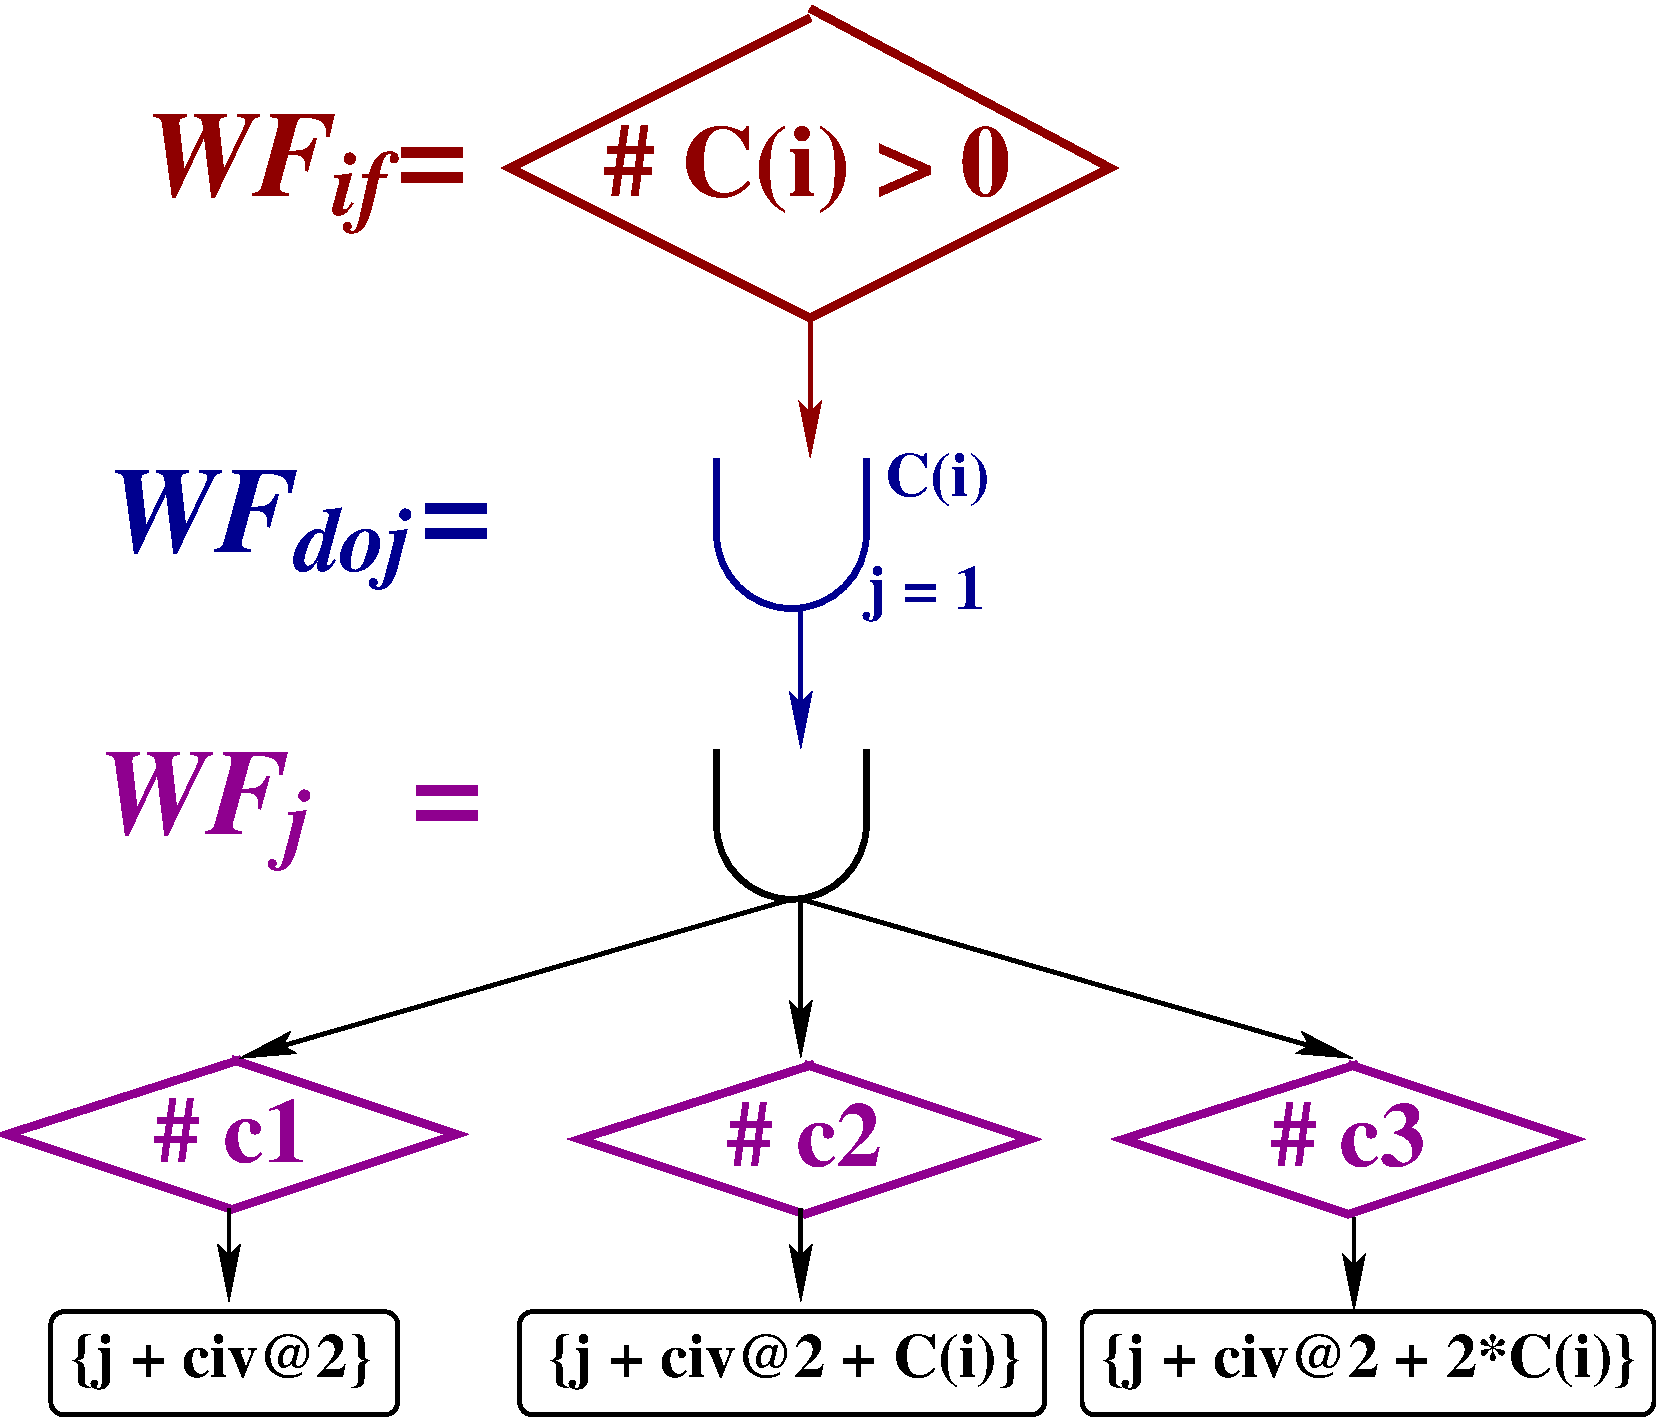
\includegraphics[height=39ex]{Figures/WFif_USR}
\end{columns}

\end{frame}



\begin{frame}[fragile,t]
\frametitle{Preliminaries: Exact (USR) Summarization (4)}

\begin{columns}
\column{0.4\textwidth}
\begin{colorcode}[fontsize=\small]
civ@1 = Q
\emphh{DO i = M, N, 1}
 civ@2=\mymath{\gamma}(civ@1,civ@4)
 .. = {\bf X}(\emp{i}) ..
 \emp{IF C(i) .GT. 0 THEN}
  \blue{DO j = 1, C(i), 1}
   \purple{IF(..)}{\bf{}X}(j+civ@2       )=..
   \purple{IF(..)}{\bf{}X}(j+civ@2+  C(i))=..
   \purple{IF(..)}{\bf{}X}(j+civ@2+2*C(i))=..
  \blue{ENDDO}
  civ@3 = 3*C(i) + civ@2
 \emp{ENDIF}
 civ@4=\mymath{\gamma}(civ@3,civ@2)
\emphh{ENDDO}
civ@5=\mymath{\gamma}(civ@4,civ@1)
\end{colorcode}
\column{0.57\textwidth}%\pause
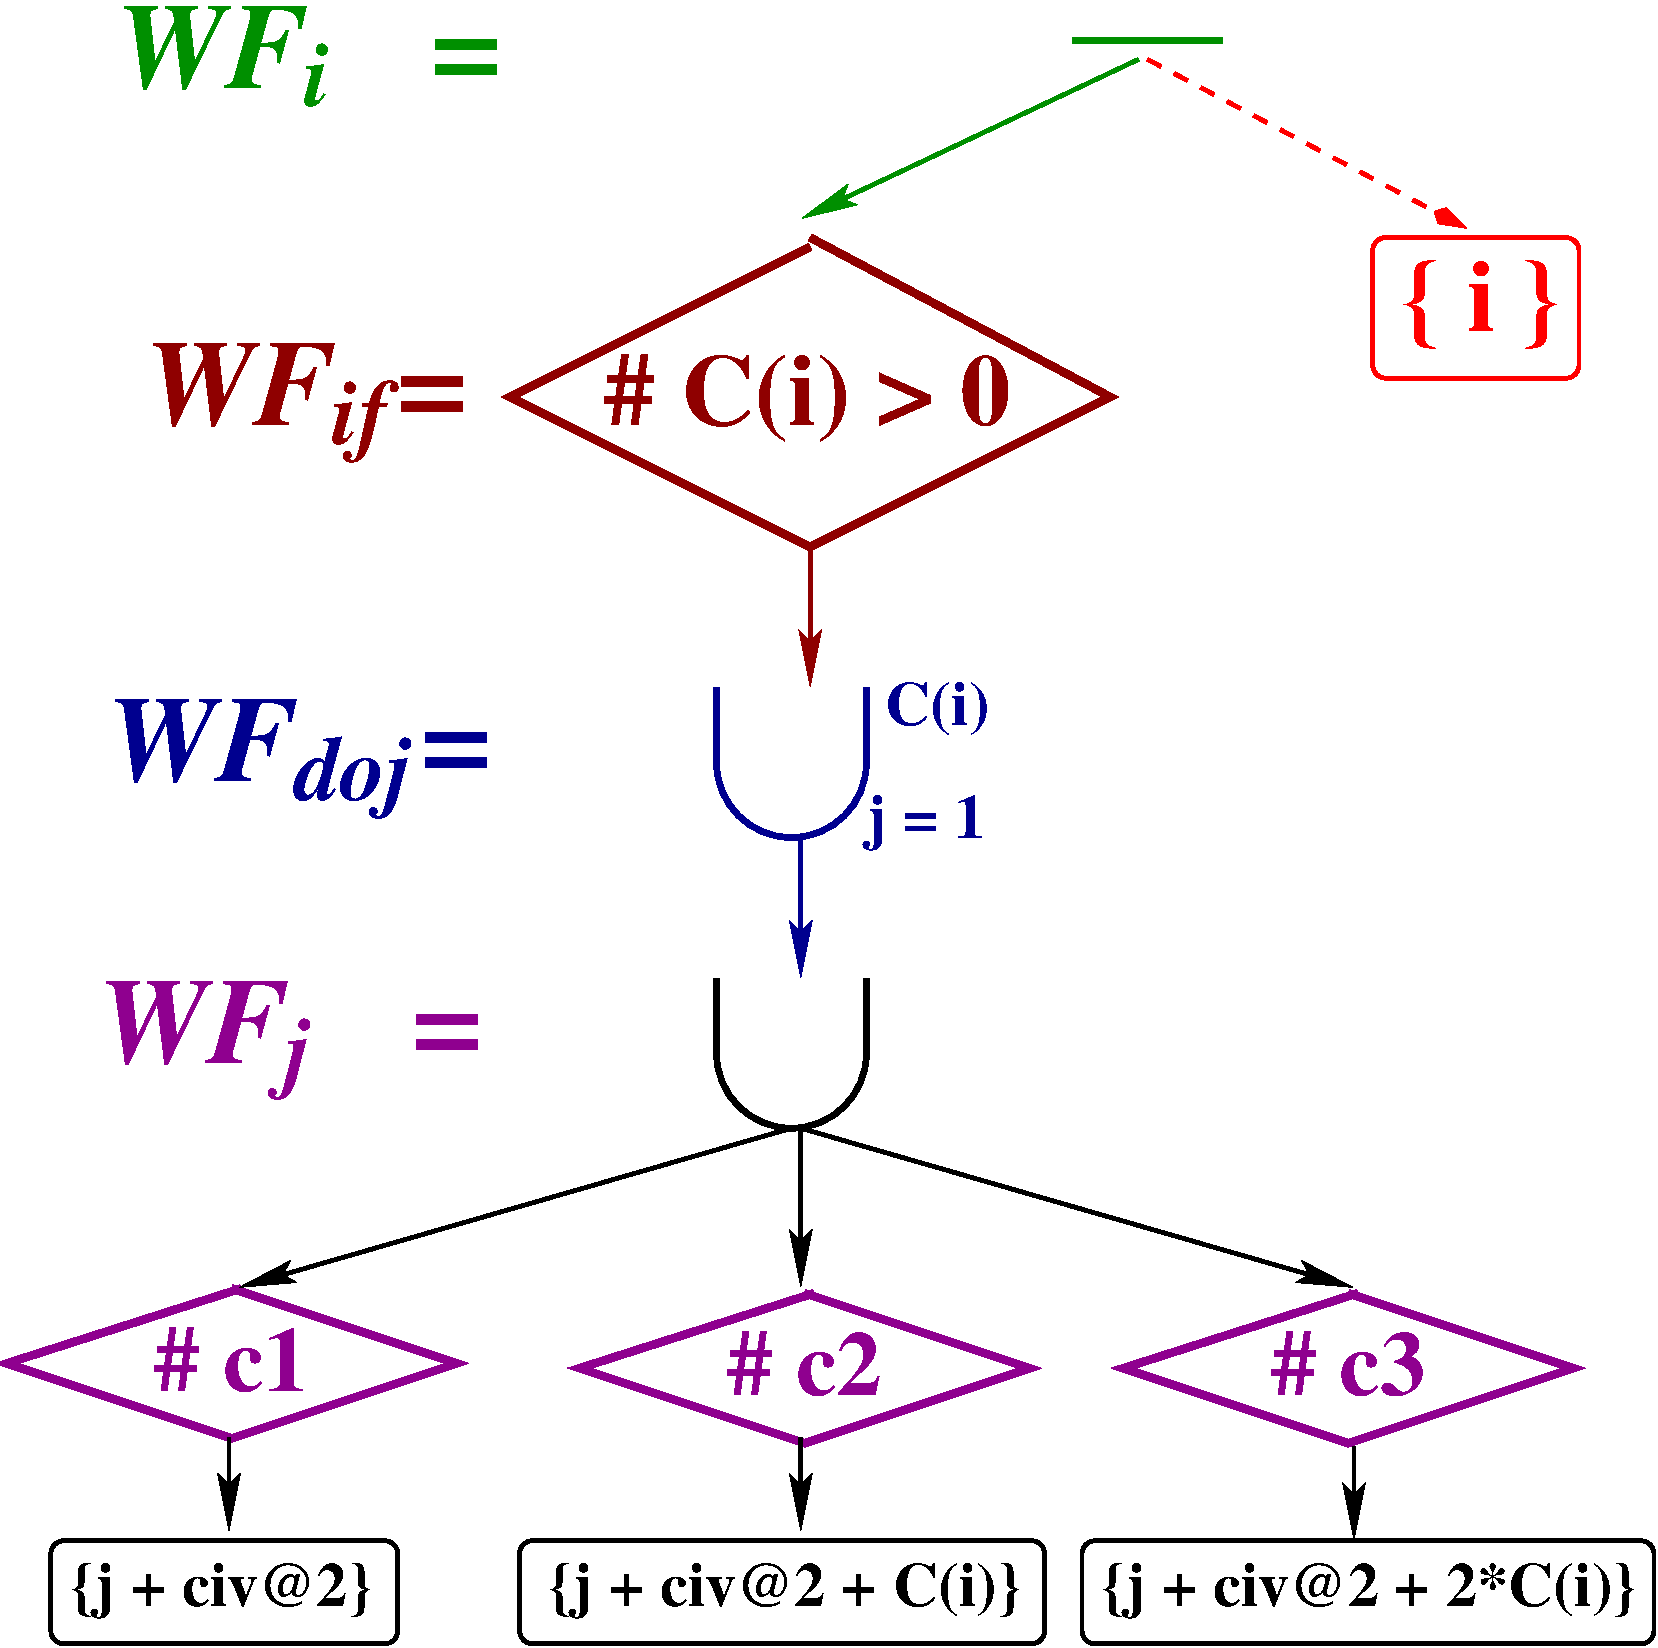
\includegraphics[height=39ex]{Figures/WFi_USR}

%\begin{itemize}
%    \item \purple{$WF_j = ${\tt{}c1\#\{j+civ@2\} $\cup$ c2\#\{j+civ@2+C(i) $\cup$ c3\#\{j+civ@2+2*C(i)\}}}\medskip\pause
%    \item \blue{$WF_{doj} = \cup_{j=1}^{C(i)} WF_j$}\medskip\pause
%    \item \emp{$WF_{if} = ${\tt(C(i).GT.0)\#$WF_{doj}$}}\medskip\pause
%    \item \emp{$RW_{if} = \emptyset$, $RO_{if} = \emptyset$}\medskip\pause
%    \item \emphh{Finally, for iteration i:}
%        \begin{itemize}
%            \item $WF_{i} = WF_{if} - \{i\}$
%            \item $RW_{i} = WF_{if} \cap \{i\}$
%            \item $RO_{i} = \{i\} - WF_{if}$
%        \end{itemize}
%\end{itemize}
\end{columns}
\bigskip\pause

\center{
\begin{huge}
\emphh{$RO_{i} = \{i\} - WF_{if}\ \& \ RW_{i} = WF_{if} \cap \{i\}$}
\end{huge}
}
\end{frame}

\begin{frame}[fragile,t]
\frametitle{Preliminaries: Value Evolution Graph (VEG)}

\begin{columns}
\column{0.49\textwidth}
\begin{colorcode}[fontsize=\small]
civ@1 = Q
DO i = M, N, 1
 \emp{civ@2=\mymath{\gamma}(civ@1,civ@4)}
 .. = {\bf X}(\emp{i}) ..
 IF C(i) .GT. 0 THEN
  DO j = 1, C(i), 1
   IF(..){\bf{}X}(j+civ@2       )=..
   IF(..){\bf{}X}(j+civ@2+  C(i))=..
   IF(..){\bf{}X}(j+civ@2+2*C(i))=..
  ENDDO
  civ@3 = 3*C(i) + civ@2
 ENDIF
 \blue{civ@4=\mymath{\gamma}(civ@3,civ@2)}
ENDDO
civ@5=\mymath{\gamma}(civ@4,civ@1)
\end{colorcode}
\column{0.54\textwidth}%\pause
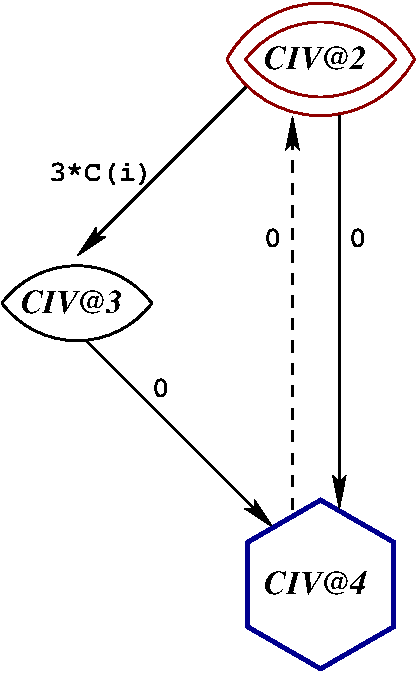
\includegraphics[height=35ex]{Figures/VEG_CORREC0.pdf}
\end{columns}
\bigskip

{\sc veg} constructed at loop and subroutine call level.\\ 
\emphh{\em Represents the flow of values between gated-SSA {\sc civ} names.} 

\end{frame}




\begin{frame}[fragile,t]
\frametitle{CIV-Summarization}

Refinement of exact summarization: computes over/underestimates\medskip
\begin{itemize}
    \item[1] Approximate {\sc usr} with a union of gated intervals.\medskip
    \item[2] Associate each gated interval with a {\sc veg} node.\medskip
    \item[3] Summarize each path in terms of start and end {\sc civ} node.
            \begin{itemize}
                \item for underestimate check that the condition of the path
                \item implies the gates of each of the interval on that path.\medskip
            \end{itemize}
    \item[4] Merge across all paths of an iteration.\medskip
    \item[5] Total/partial aggregation across loops.
\end{itemize}
\end{frame}

\begin{frame}[fragile,t]
\frametitle{1. Union of Gated-Intervals Approximation}
\bigskip

\begin{columns}
\column{0.52\textwidth}
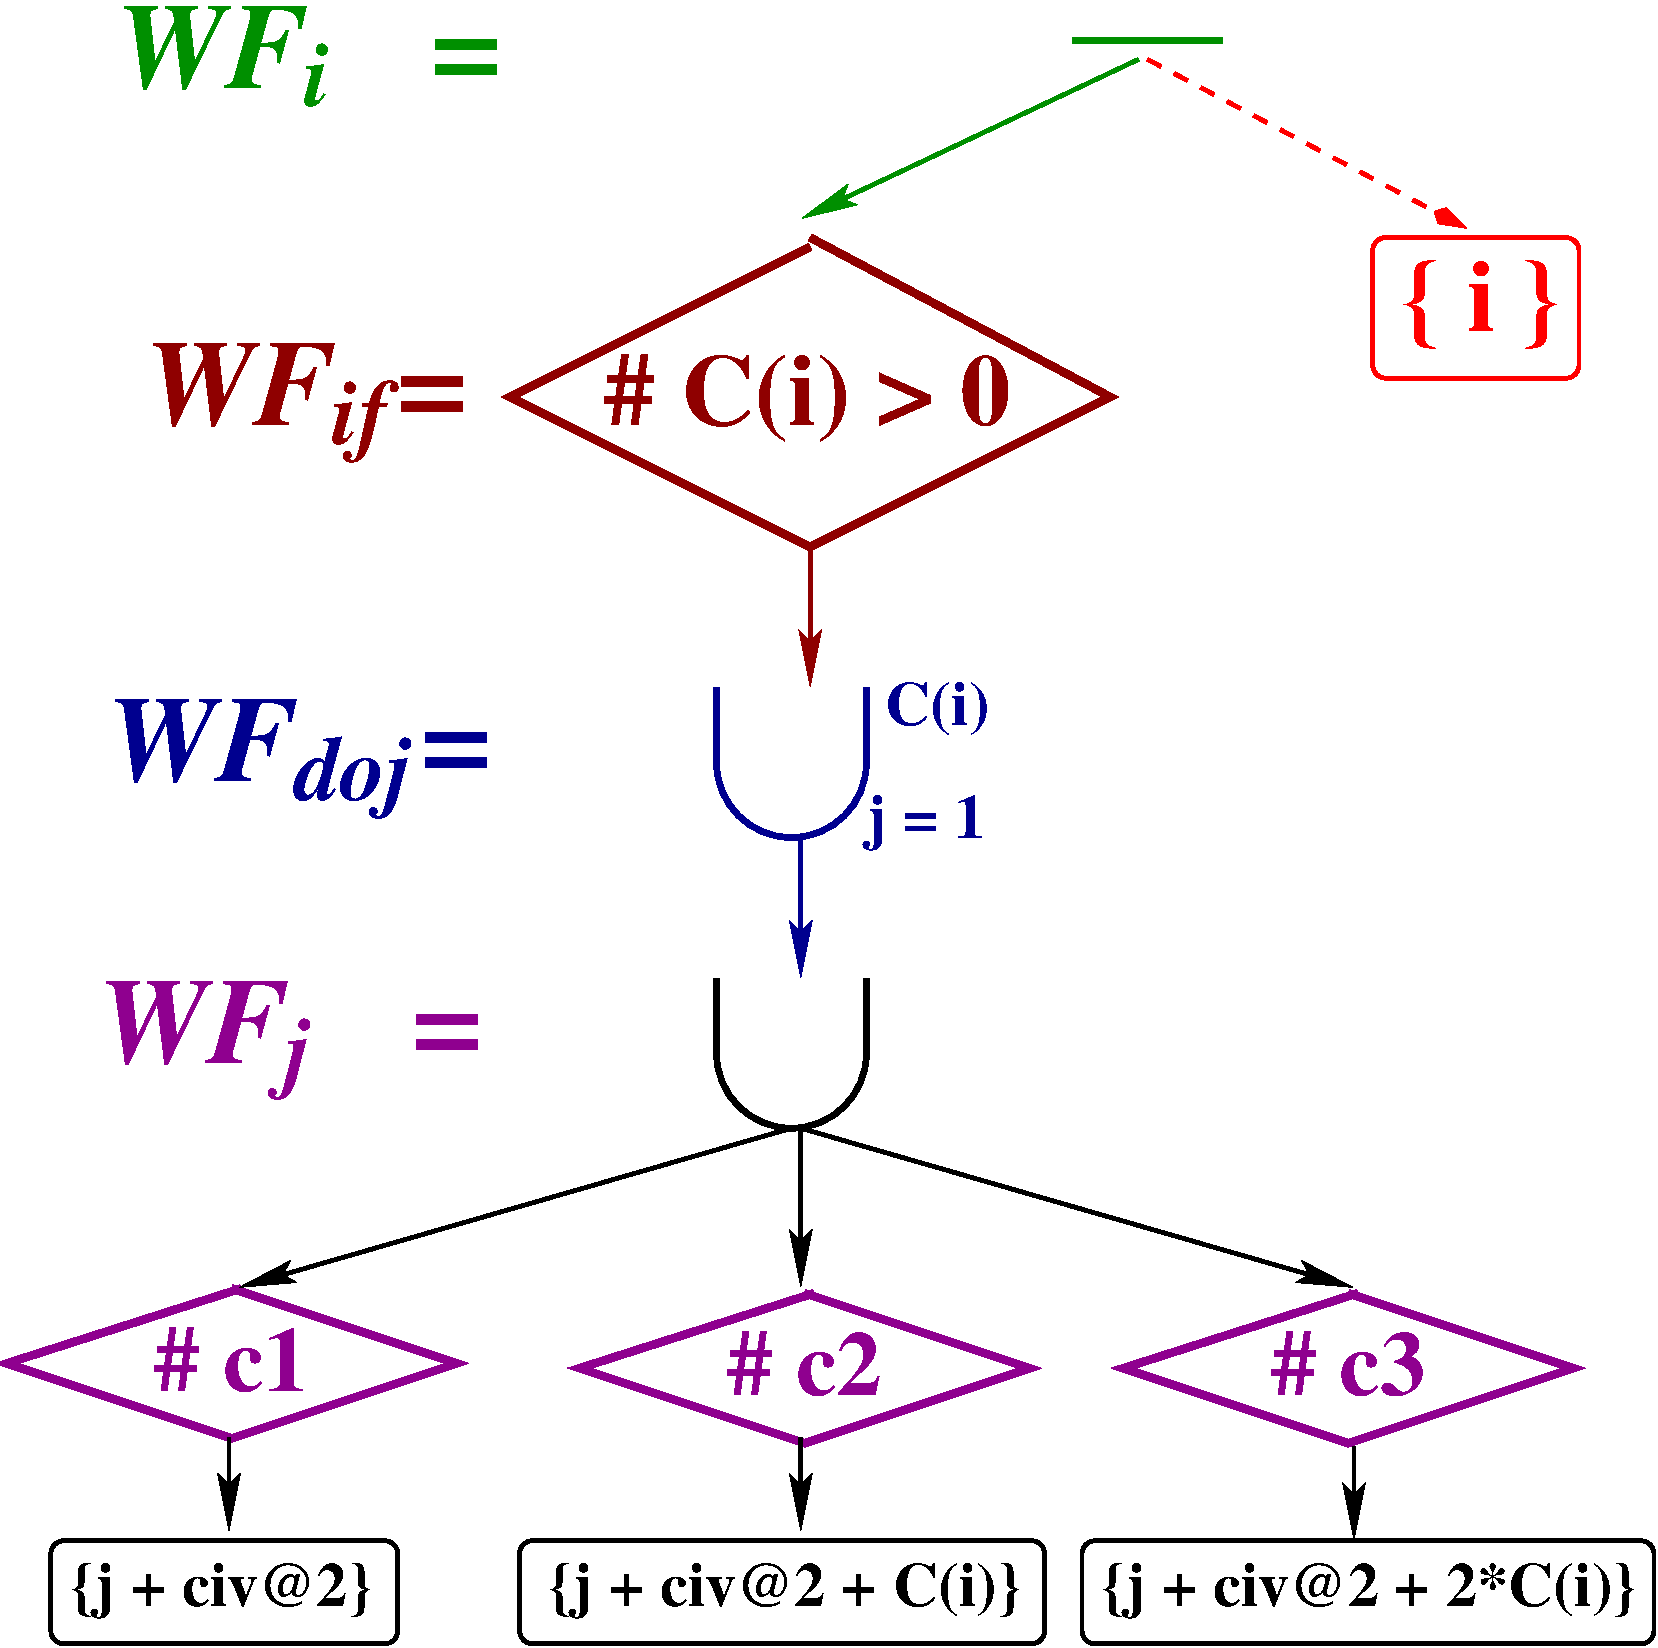
\includegraphics[height=33ex]{Figures/WFi_USR}
\column{0.46\textwidth}%\pause
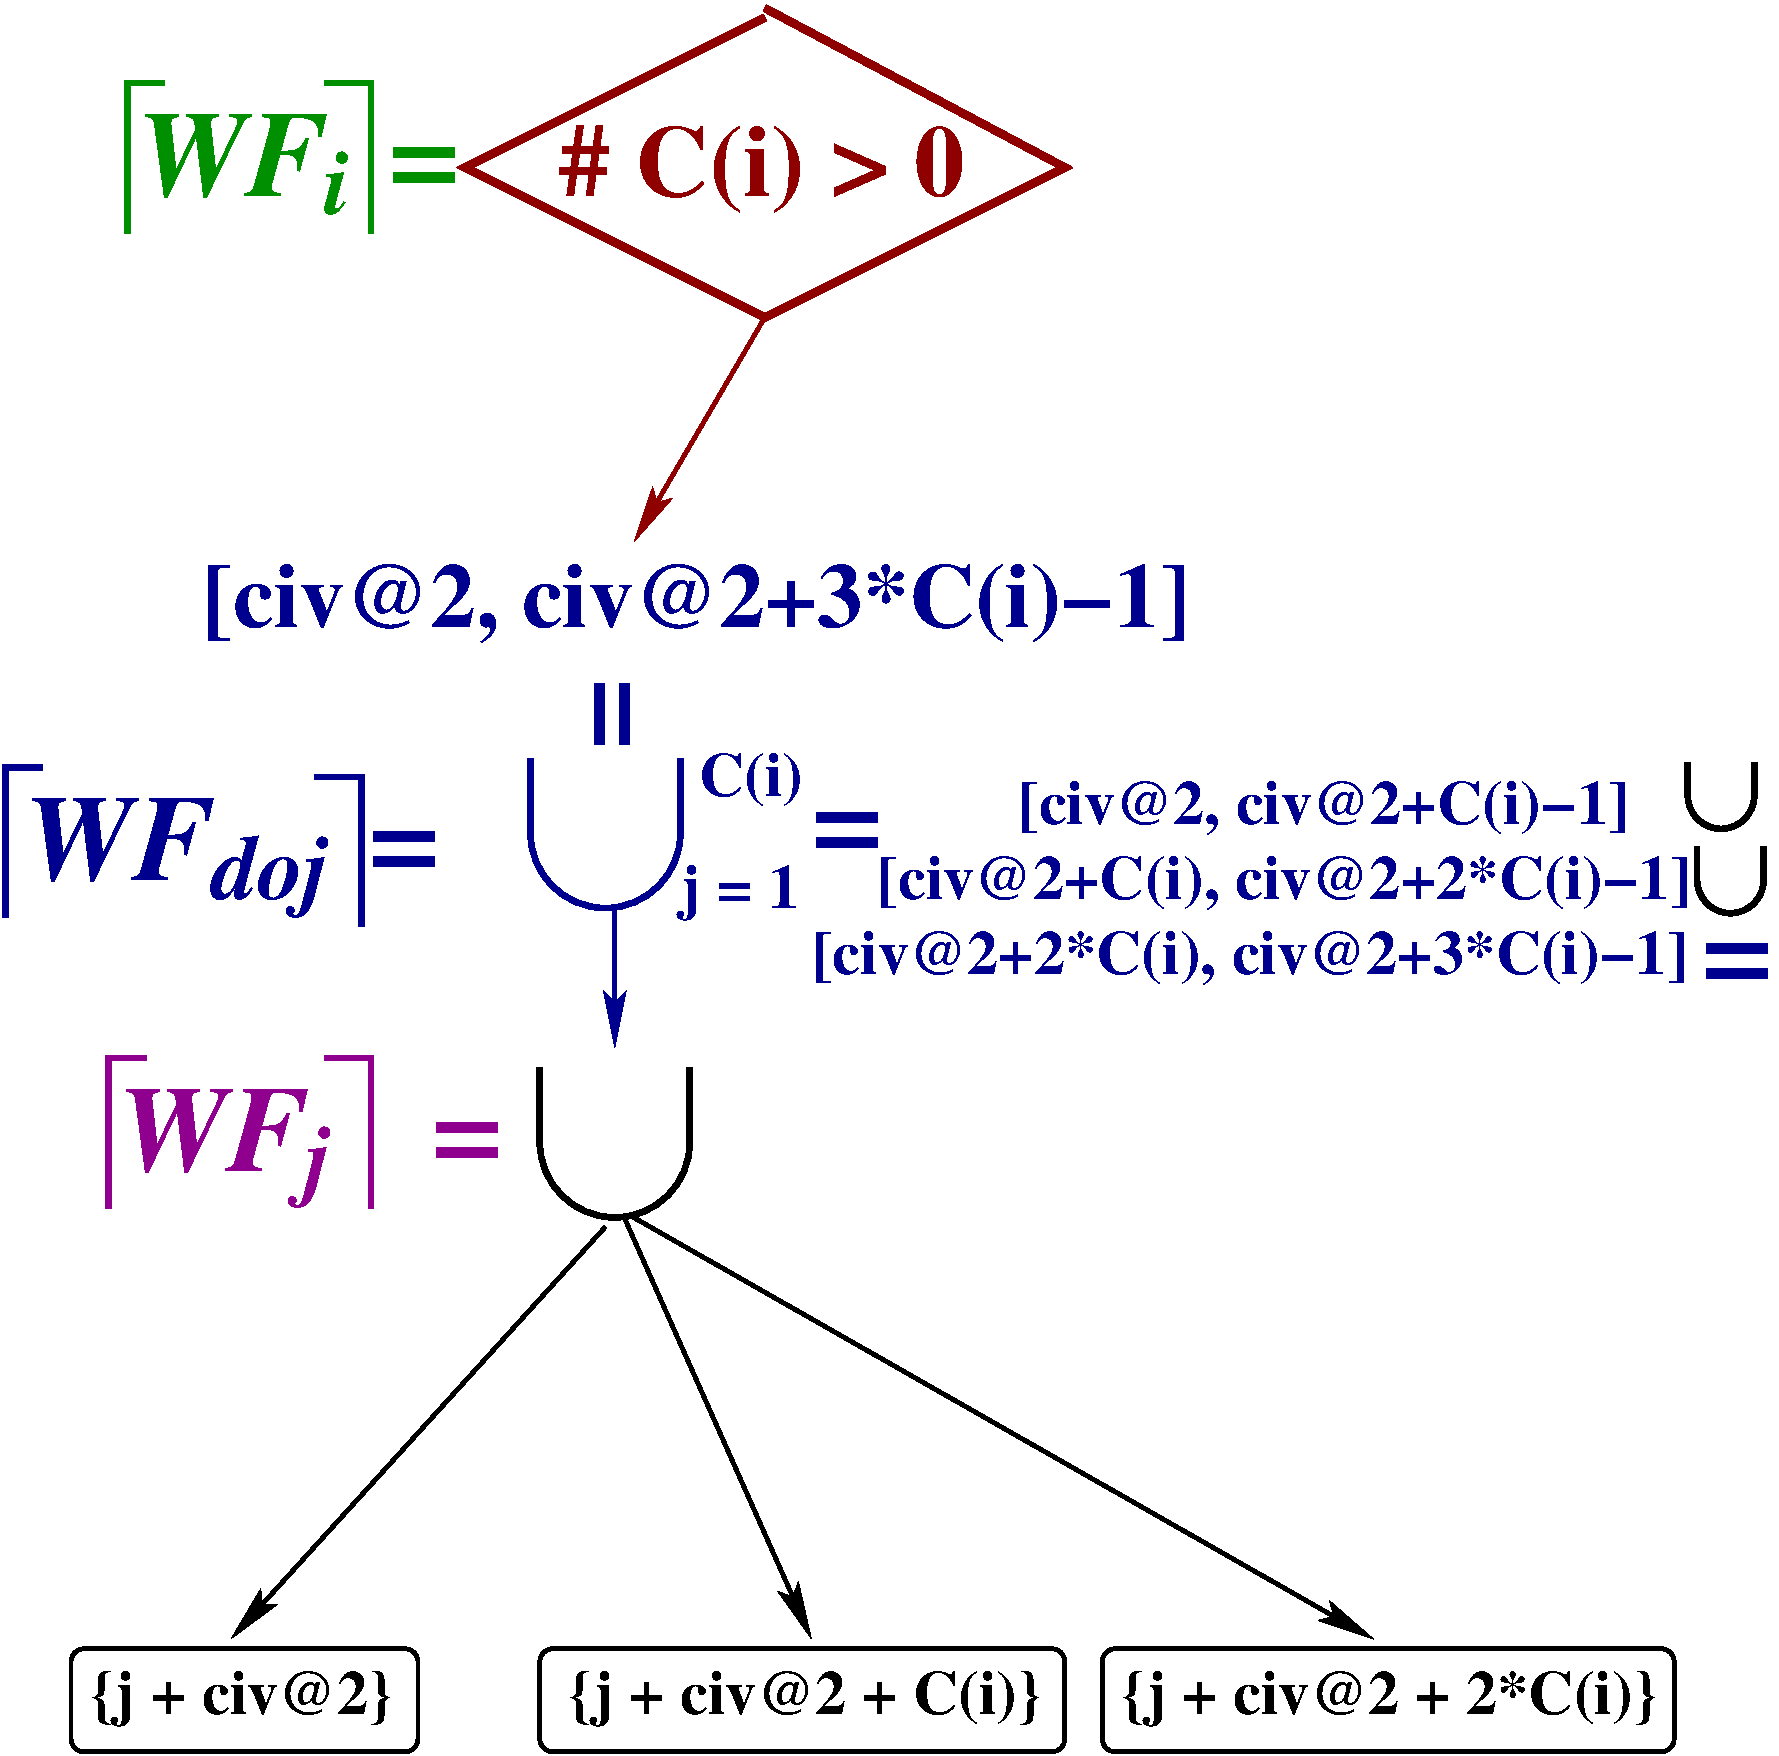
\includegraphics[height=33ex]{Figures/WFi_OVER}
\end{columns}

\end{frame}


\begin{frame}[fragile,t]
\frametitle{1. Union of Gated-Intervals Approximation}
\bigskip

\begin{columns}
\column{0.42\textwidth}
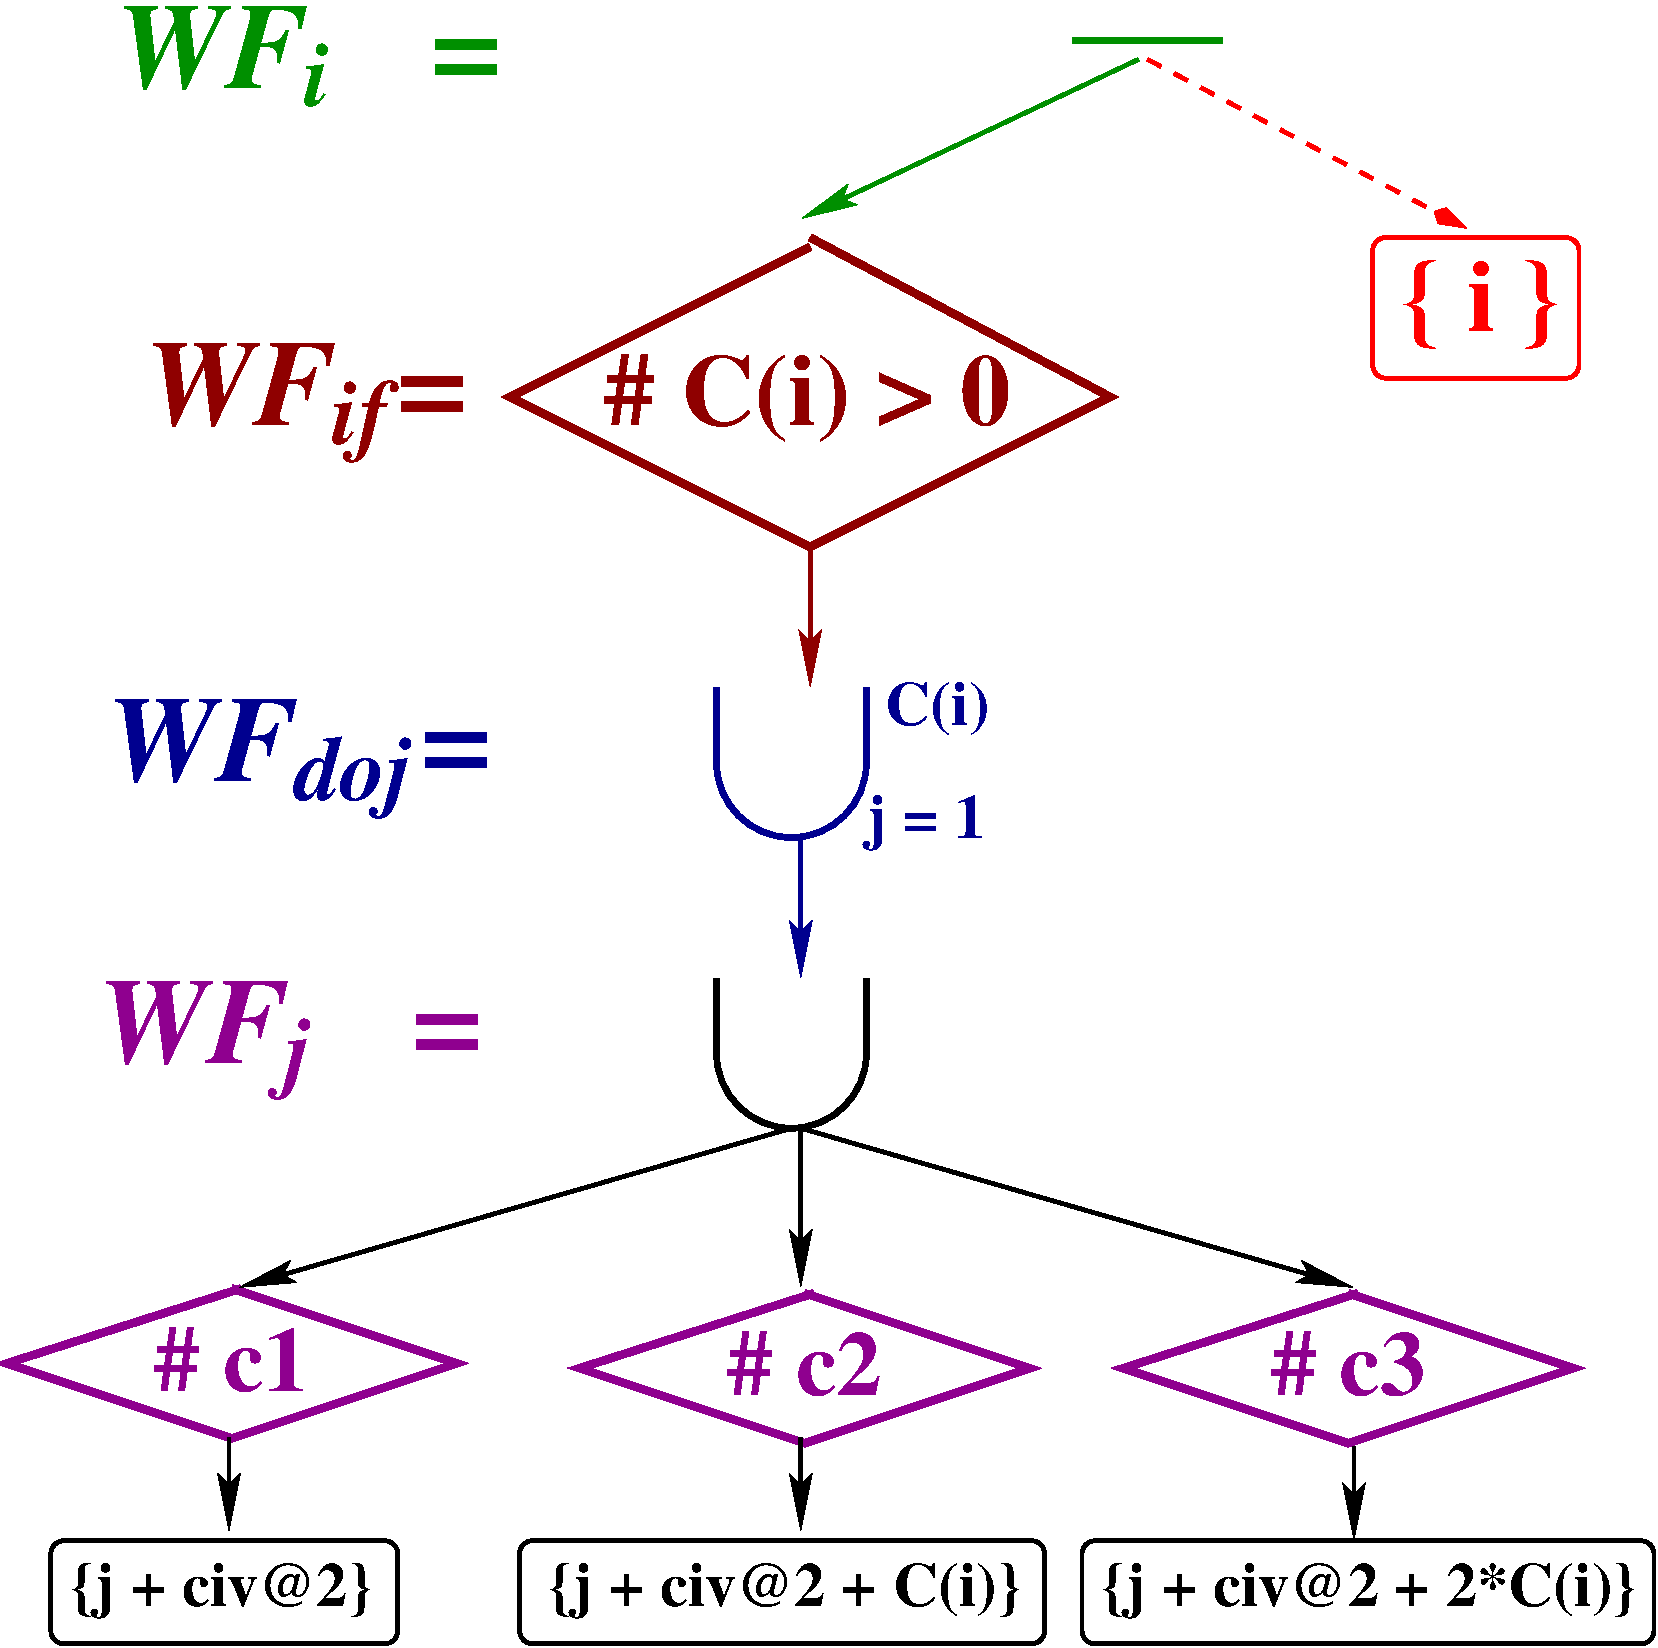
\includegraphics[height=33ex]{Figures/WFi_USR}
\column{0.56\textwidth}%\pause
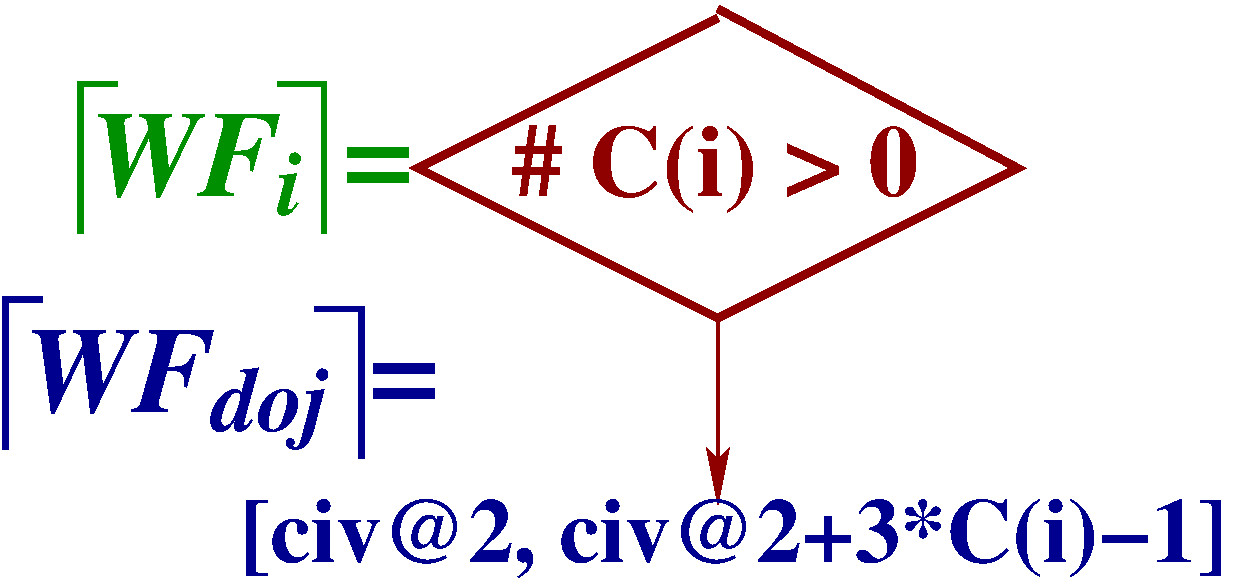
\includegraphics[height=19ex]{Figures/WFi_OVERsimpl}
\end{columns}

\end{frame}


%\begin{frame}[fragile,t]
%\frametitle{1. Union of Gated-Intervals Approximation}
%
%\begin{columns}
%\column{0.40\textwidth}
%\begin{colorcode}[fontsize=\small]
%civ@1 = Q
%\emphh{DO i = M, N, 1}
% civ@2=\mymath{\gamma}(civ@1,civ@4)
% .. = {\bf X}(\emp{i}) ..
% \emp{IF C(i) .GT. 0 THEN}
%  \blue{DO j = 1, C(i), 1}
%   \purple{IF(..)}{\bf{}X}(j+civ@2       )=..
%   \purple{IF(..)}{\bf{}X}(j+civ@2+  C(i))=..
%   \purple{IF(..)}{\bf{}X}(j+civ@2+2*C(i))=..
%  \blue{ENDDO}
%  civ@3 = 3*C(i) + civ@2
% \emp{ENDIF}
% civ@4=\mymath{\gamma}(civ@3,civ@2)
%\emphh{ENDDO}
%civ@5=\mymath{\gamma}(civ@4,civ@1)
%\end{colorcode}
%\column{0.58\textwidth}%\pause
%ToDo: replace with figures\medskip
%\begin{itemize}
%    \item \purple{$\lceil WF_j \rceil= ${\tt{}c1\#\{j+civ@2\} $\cup$ c2\#\{j+civ@2+C(i) $\cup$ c3\#\{j+civ@2+2*C(i)\}}}\medskip\pause
%    \item \blue{$\lceil WF_{doj} \rceil = ${\tt[civ@2,civ@2+3*C(i)-1]}}\medskip\pause
%    \item \emp{$\lceil WF_{if} \rceil = ${\tt(C(i).GT.0)\#}}\\
%            \emp{$\mbox{~~~~~~~~~~}${\tt[civ@2,civ@2+3*C(i)-1]}}\medskip\pause
%    \item \emp{$RW_{if} = \emptyset$, $RO_{if} = \emptyset$}\medskip\pause
%    \item \emphh{Finally, for iteration i:}
%        \begin{itemize}
%            \item $\lceil WF_{i} \rceil= ${\tt(C(i).GT.0)\#}\\
%                    $\mbox{\tt~~~~}${\tt[civ@2,civ@2+3*C(i)-1]}
%            \item $\lceil RO_{i} \rceil = ${\tt \{i\}}
%            \item $\lceil RW_{i} \rceil= ${\tt \{i\}} or $WF_i$ 
%        \end{itemize}
%\end{itemize}
%\end{columns}
%
%\end{frame}



\begin{frame}[fragile,t]
\frametitle{2. Project Gated Intervals to VEG Nodes}

\begin{columns}
\column{0.45\textwidth}
\begin{colorcode}[fontsize=\small]
civ@1 = Q
DO i = M, N, 1
 civ@2=\mymath{\gamma}(civ@1,civ@4)
 .. = {\bf X}(\emp{i}) ..
 IF C(i) .GT. 0 THEN
  DO j = 1, C(i), 1
   \purple{IF(..)}{\bf{}X}(\emp{j+civ@2       })=..
   \purple{IF(..)}{\bf{}X}(\emp{j+civ@2+  C(i)})=..
   \purple{IF(..)}{\bf{}X}(\emp{j+civ@2+2*C(i)})=..
  ENDDO
  \blue{civ@3 = 3*C(i) + civ@2}
 ENDIF
 civ@4=\mymath{\gamma}(civ@3,civ@2)
ENDDO
civ@5=\mymath{\gamma}(civ@4,civ@1)
\end{colorcode}
\column{0.55\textwidth}%\pause
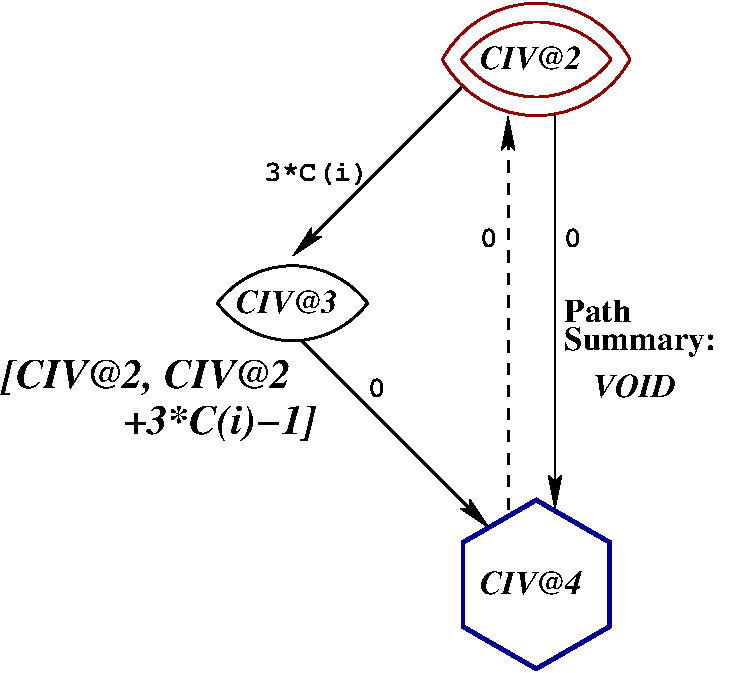
\includegraphics[height=35ex]{Figures/VEG_CORREC1.pdf}
\end{columns}
\medskip

\emphh{\em Find the {\sc civ} node that describes best the 
summarization program point: either the ``immediate'' {\sc civ}-node 
dominator or postdominator.}
%\begin{itemize}
%    \item if dominator dominates postdominator $\Rightarrow$ chose postdominator {\sc civ} node.
%    \item otherwise chose the dominator {\sc civ} node.
%\end{itemize} 


\end{frame}


\begin{frame}[fragile,t]
\frametitle{3,4. Summarize and Merge Paths}

\begin{columns}
\column{0.44\textwidth}
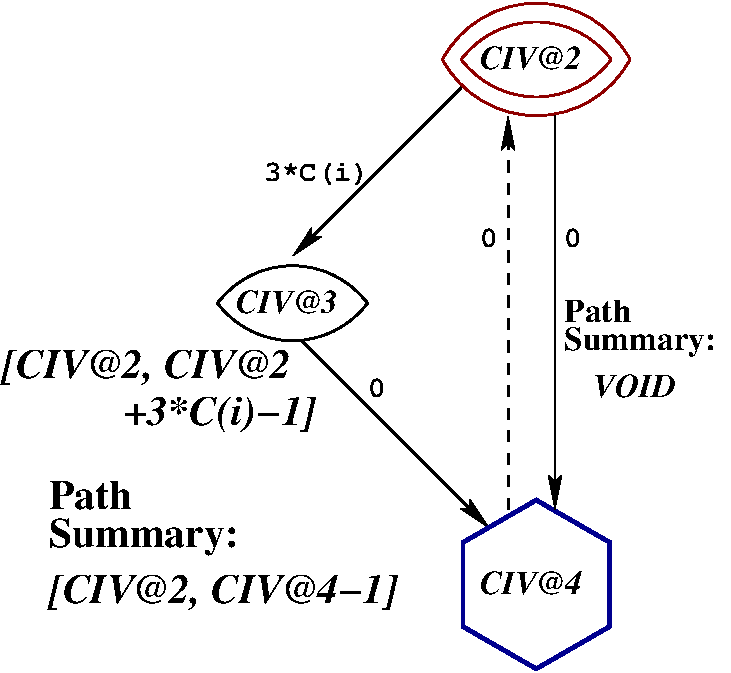
\includegraphics[height=35ex]{Figures/VEG_CORREC2.pdf}
\column{0.54\textwidth}%\pause
\begin{itemize}
    \item[1] express each path summary in terms of {\tt civ@2} and {\tt civ@4}
    \begin{itemize}
        \item[a] {\tt then} path:\\
                    {\tt [civ@2,civ@2+3*C(i)-1]\\
                    $\equiv$\emphh{[civ@2,civ@4-1]}}
        \item[b] {\tt else path:}\\
                    {\tt $\emptyset$ $\equiv$ \emphh{[civ@2,civ@4-1]}},\\
                    because {\tt civ@2 > civ@4-1}\\(0 evolution).
    \end{itemize}\bigskip\pause
    \item[2] Identical Formula, hence $\lceil WF_i \rceil = ${\tt [civ@2,civ@4-1]}
\end{itemize}
\end{columns}

\end{frame}


\begin{frame}[fragile,t]
\frametitle{5. Total Partial Aggregation Across Loop}

\begin{columns}
\column{0.33\textwidth}
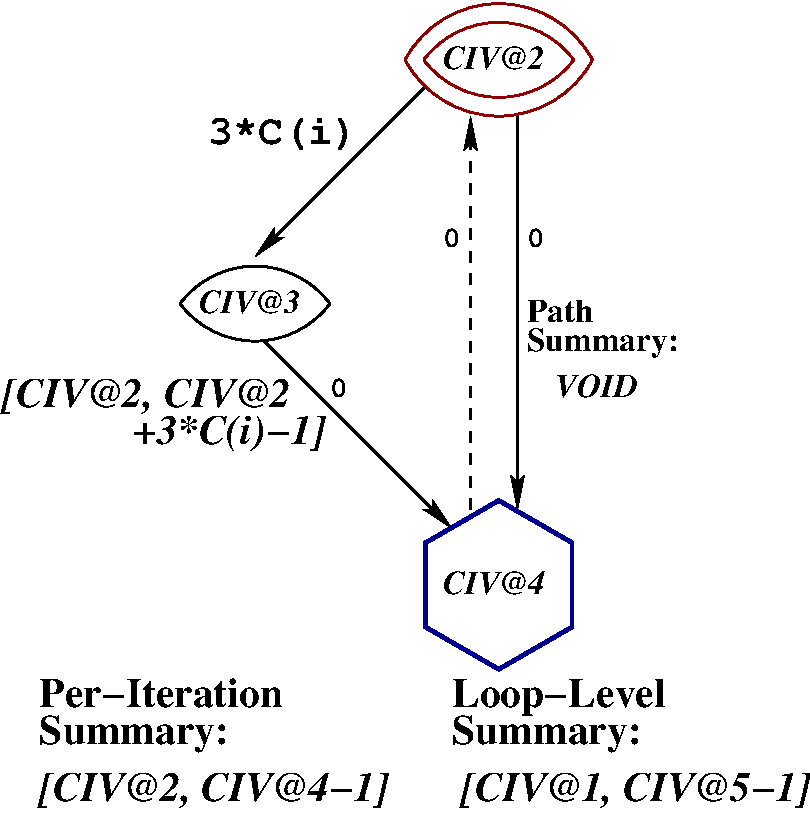
\includegraphics[height=30ex]{Figures/VEG_CORREC.pdf}
\column{0.68\textwidth}
\begin{itemize}
    \item[1] express each path summary in terms of {\tt civ@2} and {\tt civ@4}
    \begin{itemize}
        \item[a] {\tt then} path:\\
                    {\tt [civ@2,civ@2+3*C(i)-1]}$\equiv$\\
                    \emphh{{\tt[civ@2,civ@4-1]}}
        \item[b] {\tt else path:} {\tt $\emptyset$ $\equiv$ \emphh{[civ@2,civ@4-1]}},
                    because {\tt civ@2>civ@4-1} (0 evol).
    \end{itemize}\bigskip
    \item[2] Identical Formula, hence $\lceil WF_i \rceil = ${\tt [civ@2,civ@4-1]}\bigskip
    \item[3] Loop: $\cup_{i=1}^{N} \lceil WF_i \rceil = $ \emphh{\tt{}[civ@1,civ@5-1]}\pause\bigskip\bigskip\bigskip
    \item[4] $\cup_{k=1}^{i-1} \lceil WF_k \rceil = $ \emphh{\tt{}[civ@1,civ@4$^{i-1}-1$]}\\
             $\mbox{~~~~~~~~~~~~~~~}=$ \emphh{\tt{}[civ@1,civ@2$^{i}-1$]}
\end{itemize}
\end{columns}

\end{frame}


\begin{frame}[fragile,t]
\frametitle{6. Satisfiability of Independence Equations}

\begin{columns}
\column{0.33\textwidth}
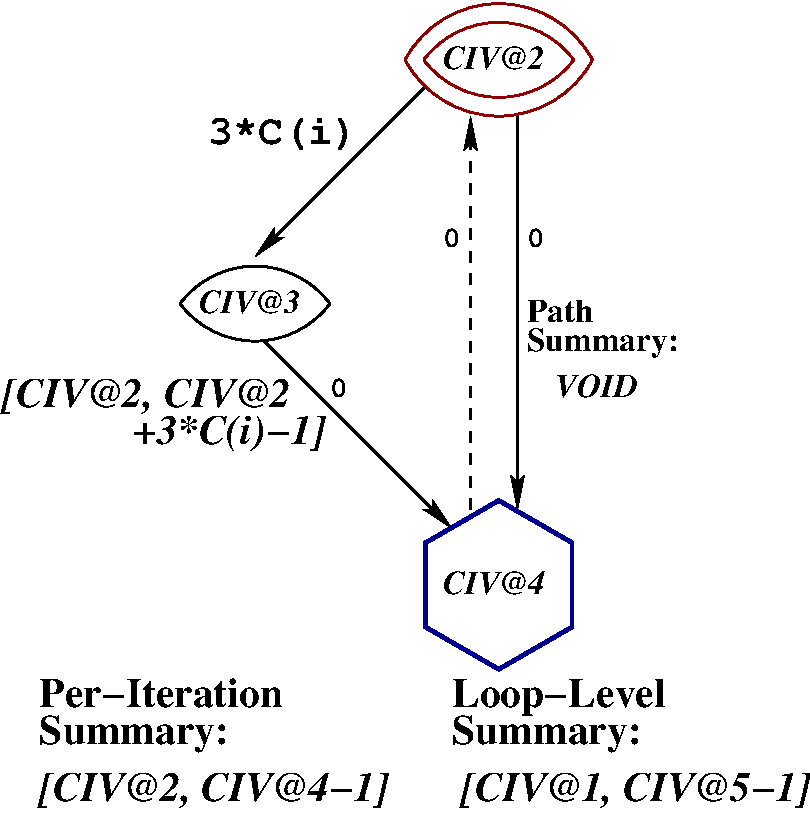
\includegraphics[height=30ex]{Figures/VEG_CORREC.pdf}
\column{0.68\textwidth}
\begin{itemize}
    \item[1] $\lceil WF_i \rceil = ${\tt [civ@2,civ@4-1]}
    \item[2] Loop: $\cup_{i=1}^{N} \lceil WF_i \rceil = $ \emphh{\tt{}[civ@1,civ@5-1]}
    \item[3] $\cup_{k=1}^{i-1} \lceil WF_k \rceil = $ \emphh{\tt{}[civ@1,civ@4$^{i-1}-1$]}\\
             $\mbox{~~~~~~~~~~~~~~}=$ \emphh{\tt{}[civ@1,civ@2$^{i}-1$]}\bigskip
    \item[4] Output independence: $\cup_{i=1}^{n}(\ \cup_{k=1}^{i-1}W_k \ \cap \ W_i ) \ = \emptyset$\smallskip\pause
    \item $\cup_{i=1}^{n}($ {\tt[civ@1,civ@2$^{i}-1$] $\cap$}\\
          $\mbox{~~~~~~~~}${\tt[civ@2$^{i}$,civ@4$^{i}-1$]$) = \emptyset$}\bigskip
\end{itemize}
\end{columns}
\bigskip
\pause

\emp{True/Anti Independence:\\
$(\cup_{i=M}^N \lceil R_i \rceil) \cap (\cup_{i=M}^N \lceil WF_i\rceil) = [M-1,N-1] \cap [civ@1, civ@5-1] = \emptyset$?}\\\medskip

\emphh{\bf Sufficient Condition:
$Q \geq N \ \vee \ M > civ@5$}

\end{frame}


\begin{frame}[fragile,t]
\frametitle{Composibility of the Technique}
\vspace{-2ex}
\begin{columns}
\column{0.49\textwidth}
\begin{colorcode}[fontsize=\small]
civ@0 = Q
\purple{DO l = 1, L}
 \emp{civ@1 = \mymath{\gamma}(civ@0,civ@5)}
 DO i = M, N, 1
  civ@2=\mymath{\gamma}(civ@1,civ@4)
  .. = {\bf X}(\emp{i}) ..
  IF C(i) .GT. 0 THEN
   DO j = 1, C(i), 1
    IF(..){\bf{}X}(j+civ@2       )=..
    IF(..){\bf{}X}(j+civ@2+  C(i))=..
    IF(..){\bf{}X}(j+civ@2+2*C(i))=..
   ENDDO
   civ@3 = 3*C(i) + civ@2
  ENDIF
  civ@4=\mymath{\gamma}(civ@3,civ@2)
 ENDDO
 \blue{civ@5=\mymath{\gamma}(civ@4,civ@1)}
\purple{ENDDO}
civ@7=\mymath{\gamma}(civ@5,civ@0)
\end{colorcode}
\column{0.54\textwidth}%\pause
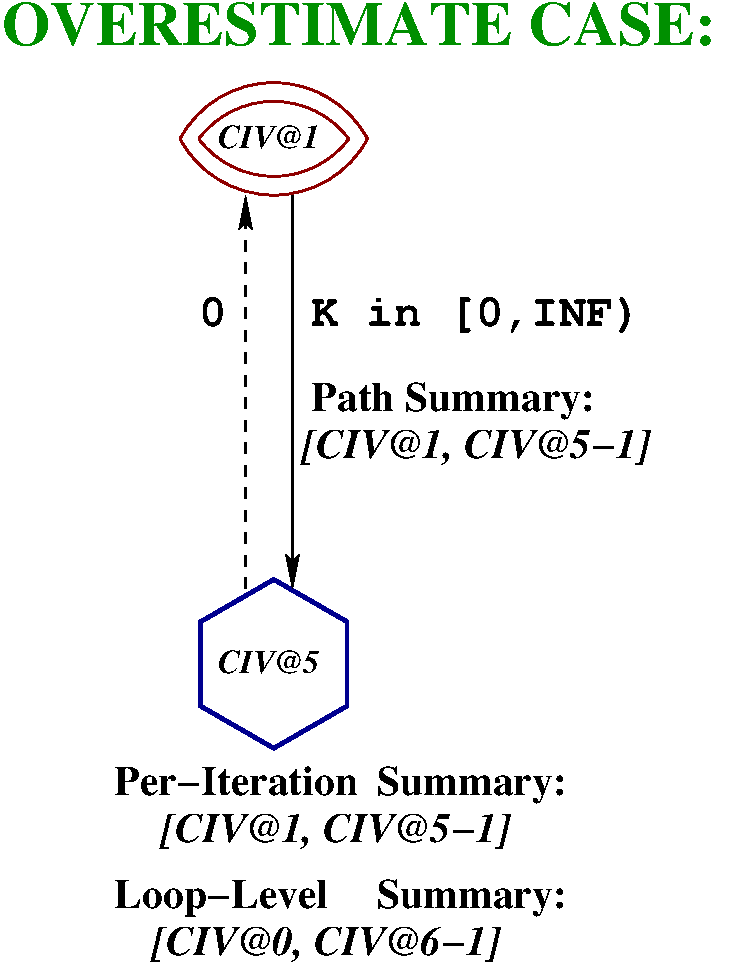
\includegraphics[height=44ex]{Figures/VEG_CORRECcomp.pdf}
\end{columns}
\bigskip

{\sc veg} constructed at loop and subroutine call level.\\ 
Represents the flow of values between gated-SSA {\sc civ} names. 

\end{frame}



\begin{frame}[fragile,t]
  \frametitle{Experimental Multi-Core Setup} \vspace{-1ex}
\bigskip

\begin{itemize}
    \item Texas A\&M's Polaris compiler $:$\\ Sequential Fortran77 $\Rightarrow$ 
            OpenMP (parallel) Fortran77.\medskip

    \item AMD Opteron(TM) 6274 system with 128GB memory.\medskip

    \item {\tt gfortran -O3}, and run on a 16-core.\medskip

    \item Empirical evaluation on $30$ {\sc perfect-club} and 
            {\sc spec} bench:\smallskip
            \begin{itemize}
                \item analyzed $2100$ loops, measured $380$ 
                        loops covering $92\%$ runtime,\smallskip
                \item \emp{Five out of thirty benchmarks ($\sim$17\%)
                        exhibit important loops that require 
                        {\sc civ}-based analysis.}
            \end{itemize}
\end{itemize}
\end{frame}


\begin{frame}[fragile,t]
\frametitle{Benchmark and Loops Characterization}
\bigskip

\begin{scriptsize}
\begin{tabular}{|c|l|l|c|c|l|} \hline
\multicolumn{6}{|c|}{Properties of Benchmarks Exhibiting Important Loops That Use {\sc civ}s} \\ \hline
{\sc bench} & {\sc properties} & {\sc do loop}  & {\sc lsc}\%  & T$_{P/S}^L$(s) & {\sc type} \\ \hline
{\sc bdna}  &  T$_{P/S}$=.19/.65 s         & {\sc actfor\_500}  & 47.8 & .05/.31 & {\sc st-par}     \\ 
{\tt P=8}         &  {\sc sc}=87\%,{\sc ov}=0\%  & {\sc actfor\_240}  & 35.6 & .04/.23 & {\sc civ}$_{\tt{}AGG}$    \\ \hline 
             &  T$_{P/S}$=1.14/3.1 s         & {\sc gmttst\_120}  & 17.4 & .27/.54 & {\sc {\sc fi} {\sc o(1)}}   \\ 
{\sc nasa7}  &  {\sc sc}=98\%,{\sc ov}=0\%  & {\sc emit\_5}      & 13.6 & .09/.42 & {\sc civ}$_{\tt{}COMP}$   \\  % ,{\sc oi} {\sc o(n)}
{\tt P=8}        &                              &                      &                & & {\sc oi} {\sc o(n)}       \\
             &                              & {\sc btrtst\_120}  & 10.1 & .05/.31 & {\sc fi} {\sc o(1)}        \\ \hline
{\sc track}  &  T$_{P/S}$=6.6/16.8 s         & {\sc fptrak\_300}  & 52.8 & 3.6/8.9 & {\sc civ}$_{\tt{}COMP}$   \\ 
{\tt P=8}        &  {\sc sc}=97\%,{\sc ov}=45\%  & {\sc extend\_400}  & 43.9 & 2.3/7.4 & {\sc civ}$_{\tt{}COMP}$ \\ \hline 
{\sc tree}   &  T$_{P/S}$=12.8/59 s        & {\sc accel\_10}    & 91.2 & 7.6/54 & {\sc civ}$_{\tt{}AGG}$  \\            %58.6%53.5
{\tt P=8}        &  {\sc sc}=91\%,{\sc ov}=0\% &                    &      &          &                           \\ \hline 
{\sc price\_i} &  T$_{P/S}$=.29/2.0 s        & {\sc price\_i\_10} & 99   & .29/2.0  & {\sc civ}$_{\tt{}AGG}$ \\ 
{\tt P=8}          &  {\sc sc}=99\%,{\sc ov}=0\% &                    &      &          &                           \\ \hline 
{\sc price\_r} &  T$_{P/S}$=.17/.98 s          & {\sc price\_r\_10}& 99   & .17/.98  & {\sc civ}$_{\tt{}COMP}$ \\ 

{\tt P=8}          &  {\sc sc}=99\%,{\sc ov}=6.4\% &                  &      &          &                          \\ \hline 
\end{tabular}
\end{scriptsize}

\end{frame}
%%%%%%%%%%%%%%%%%%%%%%%%%%%%%%%%%%%%%%%%%%%%%%%%%%%%%%%%%%%%%%%%%%
%%%%%%% DOCUMENT ENDS HERE!
%%%%%%%%%%%%%%%%%%%%%%%%%%%%%%%%%%%%%%%%%%%%%%%%%%%%%%%%%%%%%%%%%%

\begin{frame}[fragile,t]
  \frametitle{Experimental Results: Perfect-Club \& SPEC Bench} \vspace{-1ex}
\begin{columns} 
\column{0.48\textwidth} 
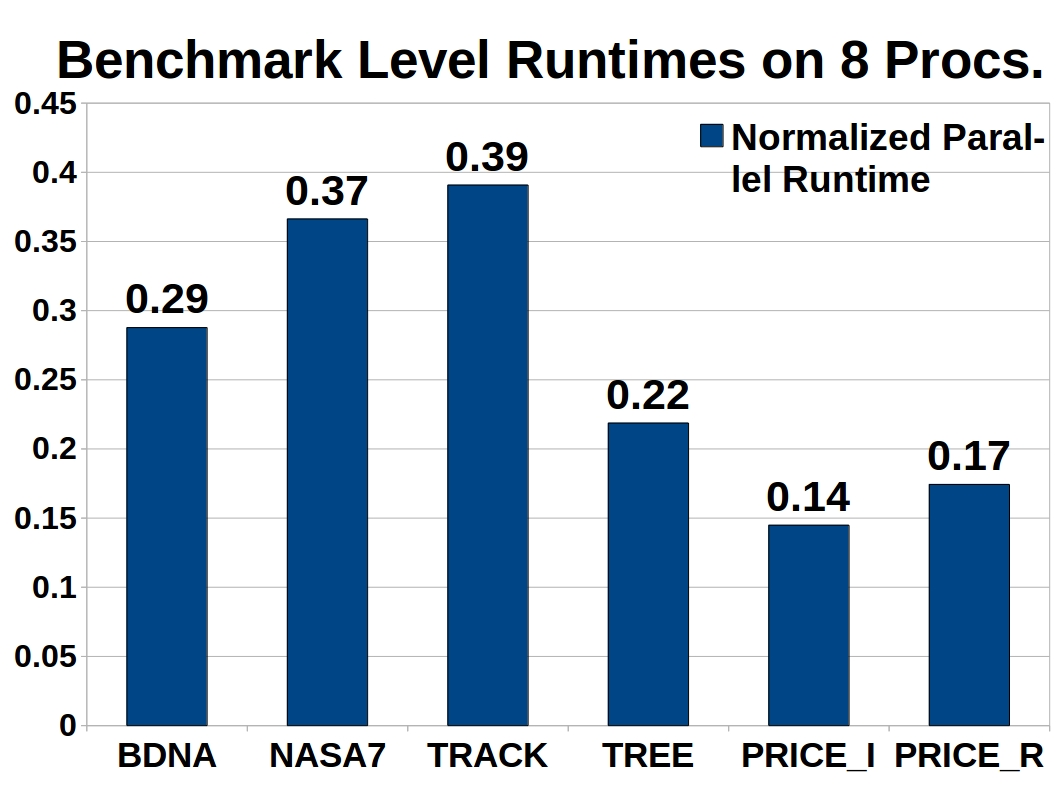
\includegraphics[width=0.95\textwidth]{Figures/EmpRes/BenchParRes.jpg}
\column{0.48\textwidth} 
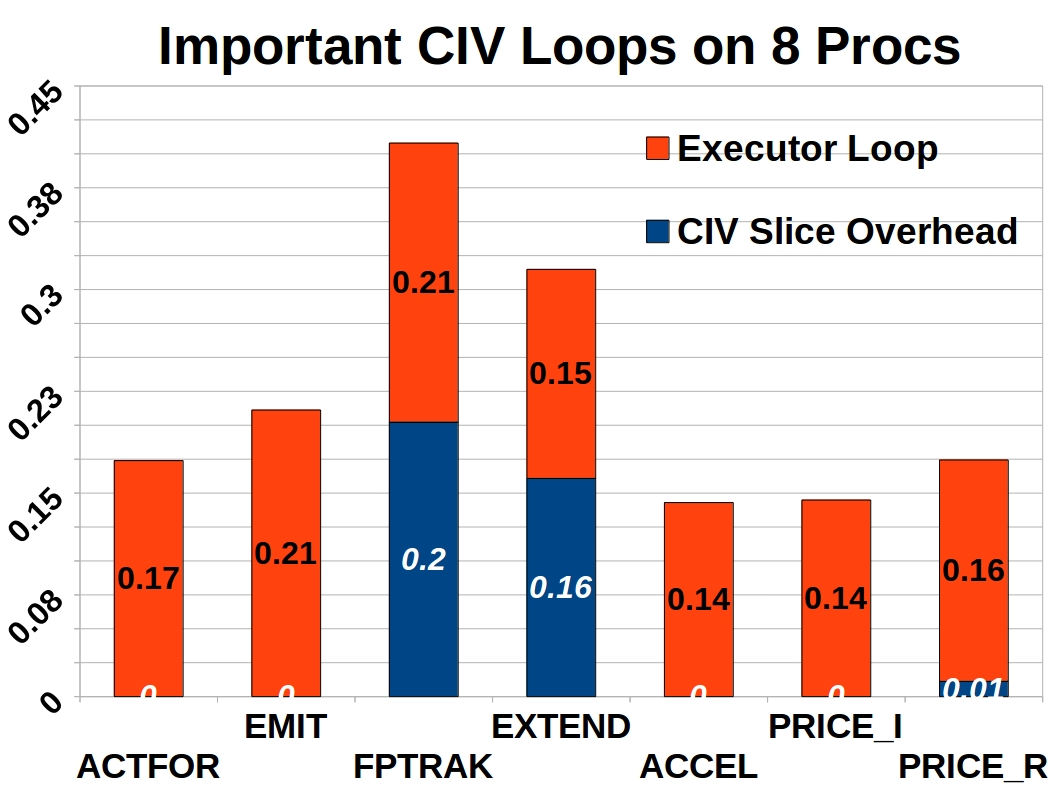
\includegraphics[width=0.95\textwidth]{Figures/EmpRes/LoopParRes.jpg} 
\end{columns}
\bigskip

\begin{columns} 
\column{0.48\textwidth} 
    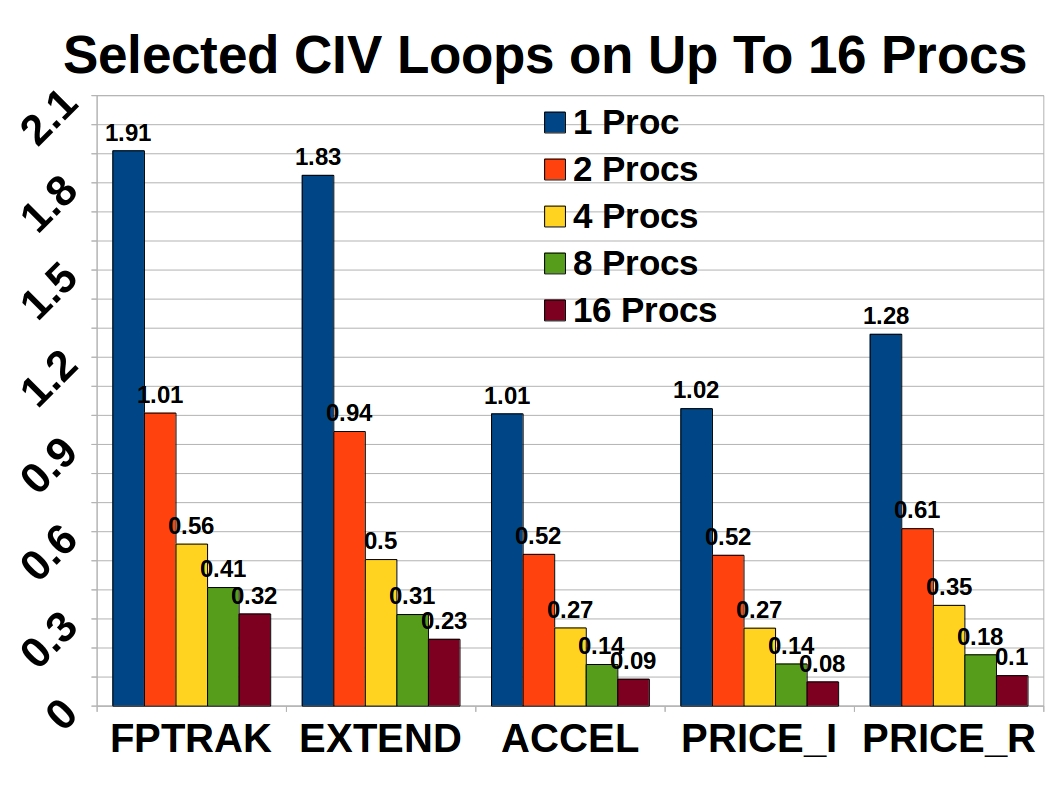
\includegraphics[width=0.95\textwidth]{Figures/EmpRes/LoopScalRes.jpg}
\column{0.48\textwidth} 
    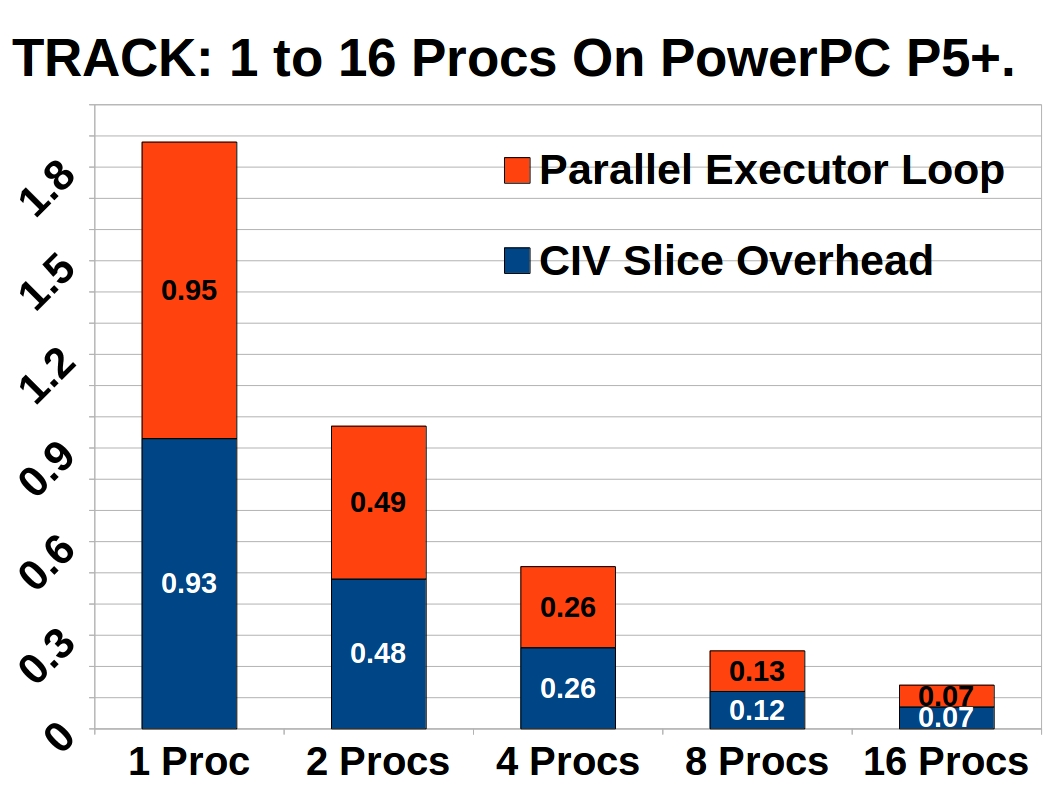
\includegraphics[width=0.95\textwidth]{Figures/EmpRes/TrackScal.jpg}
\end{columns}

\end{frame}




%\begin{frame}[fragile]
%	\tableofcontents
%\end{frame}
%\section{Auto Parallelization for Imperative Languages (Fortran77)}


\end{document}
